\documentclass{EPL-master-thesis-covers-FR}

\title{HaïtiWater 2.0}
\subtitle{Evolution de l'application HaïtiWater vers une application entièrement fonctionnelle hors-ligne}

\author{Vincent \textsc{Gradzielewski}}% Handcrafted third author :D

\degreetitle{Master [120] en sciences informatiques}

\supervisor{Kim \textsc{Mens}}
\secondsupervisor{Sandra \textsc{Soares-Frazão}}

\readerone{Celine Deknop}
\readertwo{Sebastien Strebelle}

\years{2020-2021}

\usepackage{subcaption}
\captionsetup{compatibility=false}
\usepackage{hyperref}
\usepackage{cite}
\usepackage{float}
\usepackage{multirow}
\usepackage{multicol}
\usepackage[final]{pdfpages}
\usepackage{booktabs}
\usepackage{multirow}
\usepackage{graphicx}
\usepackage{comment}
\usepackage[toc]{multitoc}
%Vérifier la table des matière (une colonne)

\usepackage{amssymb}% http://ctan.org/pkg/amssymb
\usepackage{pifont}% http://ctan.org/pkg/pifont
\newcommand{\cmark}{\ding{51}}% pour les checkmark
\newcommand{\xmark}{\ding{55}}%

\frenchbsetup{StandardLists=true} % Resolves conflict between babel and enumitem
\usepackage{enumitem} % better formating of lists

\usepackage[style=long,nonumberlist,toc,xindy,acronym,nomain]{glossaries}
%Vé
\makenoidxglossaries
	\PrerenderUnicode{Ãĺ}
	\newacronym{pwa}{PWA}{Progressive Web App}
	\newacronym{sgbd}{SGBD}{Système de Gestion de Base de Données}
	\newacronym{ueh}{UEH}{Université d'Etat de Haïti}
	\newacronym{orm}{ORM}{Object Relational Mapping}
	\newglossaryentry{full_stack}{name={Full-stack},  description={Développement à la fois sur le fontend et le backend}}
	\newglossaryentry{ong}{name={ONG}, description={Organisme financé essentiellement par des dons privés, qui se consacre à l'action humanitaire}}  
	\newglossaryentry{ares}{name={ARES-CDD}, description={L’ARES est la fédération des établissements d’enseignement supérieur de la Fédération Wallonie-Bruxelles}}
	\newglossaryentry{moscow}{name={Moscow}, description={La méthode MoSCoW est une technique visant à prioriser des besoins ou des exigences en matière d'assistance à maîtrise d'ouvrage et de développement logiciel}}
	\newglossaryentry{json}{name={JSON}, description={Format de données textuelles qui permet de représenter l'information sous forme de texte}}
	\newglossaryentry{framework}{name={Framework}, description={Ensemble cohérent de composants logiciels structurels, qui sert à créer les fondations ainsi que les grandes lignes de tout ou d’une partie d'un logiciel}}
	\newglossaryentry{django}{name={Django}, description={Django est un framework Python de haut niveau, permettant un développement rapide de sites internet, sécurisés et maintenables}}
	\newglossaryentry{postgres}{name={PostGreSQL}, description={PostgreSQL est un système de gestion de base de données relationnelle orienté objet puissant et open source}}
	\newglossaryentry{orm2}{name={Object Relational Mapping}, description={Les ORM sont des frameworks qui, comme l’indique leur nom, permettent de créer une correspondance entre un modèle objet et un modèle relationnel de base de données}}
	\newglossaryentry{postgis}{name={PostGis}, description={Extension de base de données spatiales pour postGreSQL}}
	\newglossaryentry{api}{name={API}, description={Une API est un ensemble de définitions et de protocoles qui facilite la création et l'intégration de logiciels d'applications}}
	\newglossaryentry{bootstrap}{name={Bootstrap}, description={Bootstrap est une collection d'outils utiles à la création du design de sites et d'applications web}}
	\newglossaryentry{middleware}{name={Middleware}, description={Logiciel tiers qui crée un réseau d'échange d'informations entre différentes applications informatiques}}
	\newglossaryentry{citizen}{name={Citizen Science}, description={Participation active des citoyens dans la récupération des informations utilisées dans l’application}}
	
	
		
	
	

\begin{document}

	\maketitle
	\tableofcontents

	\setlength{\parskip}{1.5em plus1em minus1em}


	\chapter*{Résumé}
	\addcontentsline{toc}{chapter}{Résumé}
	
		%Objectif, solution, évaluation
	
		Ce travail de fin d'études a été réalisé dans le cadre de mon Master en Sciences Informatiques à l'École Polytechnique de Louvain durant l'année académique 2020-2021 en partenariat avec l'\gls{ong} Protos.
		
		Dans ce mémoire, je vais vous présenter mon travail qui consistait à reprendre l'application HaïtiWater développée précedemment par Adrien Hallet, Céline Deknop et Sébastien Strebelle; "La gestion du réseau de distribution d'eau potable en Haïti" \cite{ref:haitiwater}. Le but de ce travail est de transformer cette web-application pour qu'elle soit entièrement utilisable \textbf{lorsque la connexion au serveur n'est pas disponible}.
	
		Cette application a pour but la gestion du réseau de distribution d'eau potable en Haïti. Je commencerai par présenter le contexte haïtien et les raisons pour lesquelles l'évolution de cette application était nécessaire. Ensuite je présenterai le principe des \gls{pwa} et pourquoi j'ai choisi d'utiliser cette technologie plûtot qu'une autre. J'aborderai par après la validation de l'application et les feedback que j'ai reçus des utilisateurs. En guise de conclusion, je dresserai une liste des améliorations possibles pour le futur développement de l'application.

		Tout le code source de l'application est disponible à cette adresse:\\ \url{https://github.com/exavince/HaitiWater}

		Si vous désirez tester l'application, il suffit de demander un login à un collaborateur et de vous rendre sur le lien suivant \url{https://haitiwater.sipr.ucl.ac.be} afin de vous connecter à l'application.
		

	\chapter*{Remerciements}
	\addcontentsline{toc}{chapter}{Remerciements}
		Dans le cadre de mon mémoire, j'ai été aidé par différentes personnes sans lesquelles la réalisation de celui-ci n'aurait pas été possible. Je souhaite donc consacrer ces quelques lignes pour les remercier.
		
		Merci aux professeurs Kim Mens et Sandra Soares-Frazão pour leur aide, leur soutien et les conseils indispensables qu'ils m'ont apportés tout au long de ce travail.
		
		Merci à l'\gls{ong} Protos qui a amené ce projet.
		
		Merci à Celine Deknop et Sebastien Strebelle pour l'aide et les conseils qu'ils m'ont apportés à différents moments de ce projet.
		
		Merci à Nahomie Labonte pour l'aide apportée au début du projet afin de bien mettre en évidence les besoins de l'application.
		
		Merci à tous les utilisateurs qui ont pris du temps pour tester l'application et me faire part de leur feedback.
		
		Merci à Thomas Van der Sypt pour ses éclaircissements d'un point de vue rédactionnel.
				
		Merci à mes parents et à mes amis qui m'ont soutenu et m'ont motivé tout au long de mon mémoire.

		

	\printnoidxglossary[title=Glossaire, toctitle=Glossaire]
	\glsaddall

	\chapter{Introduction}

		
		\subsection*{Contexte}
		
			Ce mémoire appartient à un projet de développement financé par \gls{ares} avec quelques partenaires tels que Protos, l'UCL et l'UEH. L'objectif de ce projet est de réaliser un système logiciel pilote pour la gestion de la distribution d'eau potable en zone rurale. C'est pour cette raison que l'\gls{ong} Protos est active en Haïti depuis plusieurs années.
			
			Protos est une \gls{ong} qui a pour but d'améliorer l'accès à l'eau potable dans plusieurs pays du monde afin de les aider à se développer. A la suite de nombreuses crises politiques et catastrophes naturelles qui ont détruit beaucoup d'infrastructures locales, l'accès à l'eau potable est devenu difficile en Haïti. De plus, des incertitudes politiques entravent la reconstruction de ces installations et les populations ne sont pas toujours aidées par les services publiques pour assurer la distribution de l'eau. 
			
			 En effet, aucune gestion centralisée et organisée par l'Etat n'existe pour les zones rurales éloignées des grandes agglomérations. Des réseaux existent, constitués de points de prélèvement d'eau, de conduites de distribution d'eau et de fontaines situées dans les villages, mais la gestion publique de ceux-ci n'est pas opérationnelle. 

			L'application créée précédemment \cite{ref:haitiwater} propose un appui à ces organismes locaux afin de mieux organiser cette distribution. 

			

		\subsection*{Problématique}
			Actuellement, HaïtiWater est une application web prévue pour fonctionner uniquement lorsque le réseau est stable et fonctionnel. Malheureusement, en Haïti, la connexion au réseau internet est assez instable, voire indisponible par endroits. Il faut donc trouver une solution pour que cette application puisse être utilisable et fiable dans les conditions du contexte haïtien. 


		\subsection*{Motivations}
			J'ai réalisé ce travail dans le cadre de mon Master en Sciences Informatiques. L'objectif est de mettre en application les différentes compétences acquises durant mes années d'étude sur un projet de grande envergure.
			
			Au-delà de mettre mes compétences en pratique, ce travail va me permettre d'acquérir de l'expérience dans le développement d'applications et surtout dans l'utilisation des nouvelles technologies du web. Il va me permettre d'apprendre à m'intégrer dans un projet de grande ampleur, de me familiariser avec un environnement logiciel déja existant et d'y apporter ma touche personnelle.	
			
			Le plus motivant dans l'évolution de cette application était de savoir qu'il s'agit d'un projet réel avec de vrais acteurs qui vont utiliser cette application sur le terrain une fois que celle-ci sera terminée.


		\subsection*{Objectifs}
			L'objectif de mon mémoire est de proposer une nouvelle version de l'application HaïtiWater afin que celle-ci soit plus adaptée à un usage sur le terrain. Normalement, cette nouvelle version devrait être déployée en Haïti cette année et ce sont les acteurs locaux qui devraient reprendre sa maintenance et son évolution.
			
			Le second objectif est de délivrer une application propre et stable qui donnera envie aux utilisateurs travaillant sur le terrain de remplacer leurs outils actuels par ce nouvel outil.
			
			
		\subsection*{Approche}
			Avant de lancer le développement de cette deuxième version de l'application, un travail d'analyse conséquent a été réalisé afin de déterminer les différentes fonctionnalités à implémenter et la technologie à utiliser. Pour ce faire, j'ai eu recours à l'analyse de \gls{moscow} \cite{ref:moscow}.
		
			Après cette phase d'analyse, je me suis lancé dans la phase de développement durant laquelle j'ai implémenté toutes les fonctions décrites lors de la phase d'analyse. Etant donné le nombre de fonctions à implémenter et la nécessité de faire de la documentation pour les futurs développeurs, cette phase a été la plus longue à réaliser.
						
			Pour finir vient la phase de validation. L'application a été présentée à des utilisateurs (certains ayant utilisés la première version, d'autres non) afin qu'ils puissent fournir le feedback nécessaire à son évolution.
			
			
		\subsection*{Contribution}
			Grâce au travail réalisé, Protos et les acteurs locaux haïtiens vont pouvoir déployer l'application et l'utiliser sur le terrain, même dans les zones les plus rurales. En effet, celle-ci peut maintenant être utilisée lorsque la connexion au serveur n'est plus disponible. Pour l'instant, ces acteurs utilisent des outils basiques tels que le crayon et le papier pour dresser leurs rapports sur le terrain. Cette outil ne permet pas un accès facile aux informations passées et complique la transmission de l'information à la hiérarchie. L'utilisation de l'application permettra de résoudre ces deux problèmes.
			
			J'espère avoir apporté ma contribution à une meilleure gestion de l'eau en Haïti en aidant à l'évolution de cette application. Pour ma part, ce travail m'aura permis d'acquérir de nouvelles compétences dans le développement \gls{full_stack} d'applications web.
			


		
%---------------------------------------------------------------------------------------------------------------
	\chapter{Contexte}


		\section{Gestion de l'eau en Haïti}
			\label{sec:situation}
			
				Haïti est l'un des pays les plus pauvres au monde. Il est situé dans une zone géographique où les risques de catastrophes naturelles sont très élevés. Ces intempéries détruisent les infrastructures et empêchent le bon développement du réseau de distribution d'eau potable. Il y a quelques années, en 2010, le pays a subi un énorme séisme qui a ravagé une bonne partie du territoire. Parmi tous les défis à relever vient celui de la gestion et de la distribution de l'eau potable, surtout dans les zones les plus rurales. Le climat de la région rendant excessivement difficile l'exploitation directe des cours d'eau, il faut beaucoup d'infrastructures afin de pouvoir assumer la distribution de l'eau potable à tous.
				
				En raison de la grande pauvreté qui règne sur la plupart de l'île et de gros problèmes organisationnels, il est très difficile de maintenir et de développer le réseau de distribution d'eau potable. Il y a un manque significatif de collaboration entre les entités haïtiennes ainsi qu'entre les villages. Ce manque est dû, en partie, à une communication non optimisée, quasi inexistante dans certains cas. Dans les zones les plus rurales de l'île, le taux de recouvrement des factures est excessivement faible, jusqu'à 11\%.
				
				Pour toutes ces raisons, l'\gls{ong} Protos vient donc en aide à Haïti afin d'aider le service national des eaux dans la gestion des infrastructures et de la facturation des clients, surtout dans les zones les plus rurales.
				
				Pour de plus amples informations sur les problèmes environnementaux, politiques, sociaux ou organisationnels du contexte haïtiens, je vous invite à consulter le mémoire Céline Deknop, Adrien Hallet, Sébastien Strebelle \cite{ref:haitiwater}.



		\section{Introduction à l'application}
				Dans le cadre de la situation décrite dans la section \ref{sec:situation}, Protos a fait appel à l'UCL afin de créer une application d'aide à la gestion et à la distribution de l'eau potable en Haïti. Une première version de l'application a été développée en 2018-2019 par trois personnes dans le cadre de leur mémoire \cite{ref:haitiwater}. Elle comprend différents modules permettant de faciliter la gestion des infrastructures et de gérer les différents consommateurs. L'application est basée sur un principe hiérarchique, la figure \ref{fig:hierarchie} démontre ce principe et provient du mémoire de Céline Deknop, Adrien Hallet, Sébastien Strebelle \cite{ref:haitiwater}.
				
				\begin{figure}[H]
					\centering
					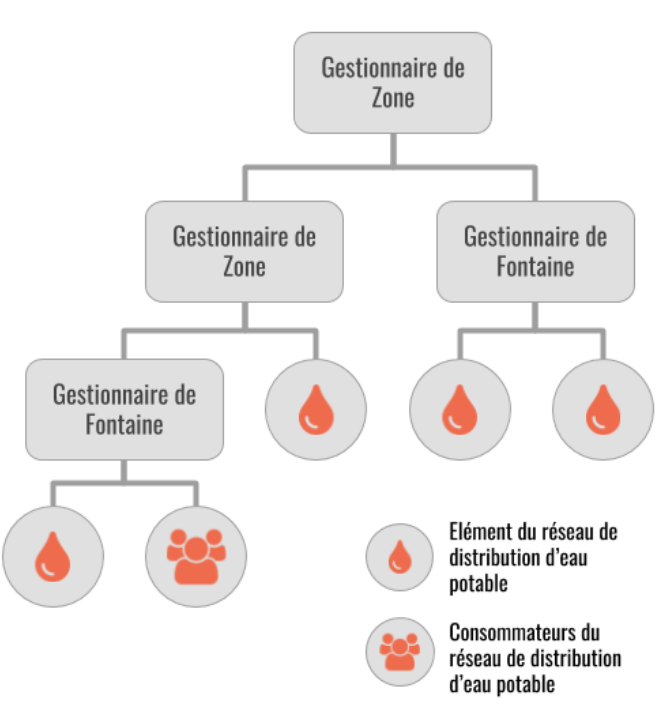
\includegraphics[width=0.5\textwidth]{images/hierarchie}
					\caption{Hiérarchie dans l'application}
					\label{fig:hierarchie}
				\end{figure}
				
				
			\subsection*{Eléments de l'application}
				\begin{description}
					\item[Zone] Une zone représente une partie du territoire. Elle peut être subdivisée en plusieurs sous-zones, la zone tutrice reprendra alors toutes les données des zones tutorées. Cela permet de séparer les responsabilités des différents territoires.
					\item[Elements du réseau] Ces éléments représentent les points physiques du réseau de distribution d'eau potable. On en dénombre six types: conduites, réservoirs, sources, fontaines, kiosques et prises individuelles. Tous ensemble, ils forment le réseau de distribution au complet. 
					\item[Consommateurs] Le consommateur est une personne qui va utiliser le réseau de distribution d'eau potable. Lors de son enregistrement, chaque consommateur se voit attribué un seul élément de sortie d'eau du réseau: fontaine, kiosque ou prise individuelle. De cette façon, il est plus simple de gérer la facturation des consommateurs.
				\end{description}
				
							
			\subsection*{Utilisateurs de l'application}
				Il y deux types d'utilisateurs qui peuvent se connecter à l'application.
				
				\begin{description}
					\item[Gestionnaire de fontaines] Ce gestionnaire va gérer la distribution de l'eau aux différents consommateurs. Il devra gérer tous les éléments du réseau qui lui sont attribués.
					\item[Gestionnaire de zones] Ce gestionnaire va avoir la responsabilité de gérer d'autres gestionnaires de zones et/ou des gestionnaires de fontaines. Sa taĉhe principale est d'administrer et de surveiller les personnes qui sont en-dessous de lui.			 
				\end{description}
				
				Ces deux gestionnaires vont avoir des privilèges différents et peuvent donc interagir différemment avec les données. Le tableau \ref{tab:permissions} provenant du mémoire de Céline Deknop, Adrien Hallet et Sébastien Strebelle \cite{ref:haitiwater} permet d'illuster plus simplement cela.
				
				\begin{table}[H]
					\centering
					\small
					\setlength\tabcolsep{2pt}
					\begin{tabular}{|l|c|c|}
						\hline
						\multirow{2}{*}{\textbf{Permission}} & \multicolumn{2}{c|}{\textbf{Gestionnaire}} \\ \cline{2-3}
						 & \textbf{fontaine} & \textbf{zone} \\ \hline
						 Ajouter/modifier/supprimer un consommateur & \cmark & \cmark \\ \hline
						 Ajouter/modifier/supprimer un élément du réseau de distribution & \cmark & \cmark \\ \hline
						 Ajouter/modifier/supprimer un rapport mensuel & \cmark & \cmark \\ \hline
						 Ajouter/modifier/supprimer un paiement & \cmark & \cmark \\ \hline
						 Ajouter/modifier/supprimer un ticket de support & \cmark & \cmark \\ \hline
						 Ajouter/modifier/supprimer une zone & \xmark & \cmark \\ \hline
						 Ajouter/modifier/supprimer un gestionnaire & \xmark & \cmark$^{*}$ \\ \hline
						 Accepter/refuser un changement dans l'historique & \xmark & \cmark \\ \hline
						 \multicolumn{3}{p{\textwidth}}{\emph{* Un gestionnaire de zone ne peut pas modifier les informations personnelles (mot de passe, courrier, nom, prénom) d'un gestionnaire existant}} \\
					\end{tabular}
					\caption{Permissions dans l'application, par type d'utilisateur}
					\label{tab:permissions}
				\end{table}
				
			
			\subsection*{Module "Accueil"}
				Ce module contient les informations condensées de la zone attribuée à l'utilisateur: le nombre de fontaines, de kiosques, de points de prises individuelles, de conduites, de foyers et de consommateurs individuels. 
								
				\begin{figure}[H]
					\centering
					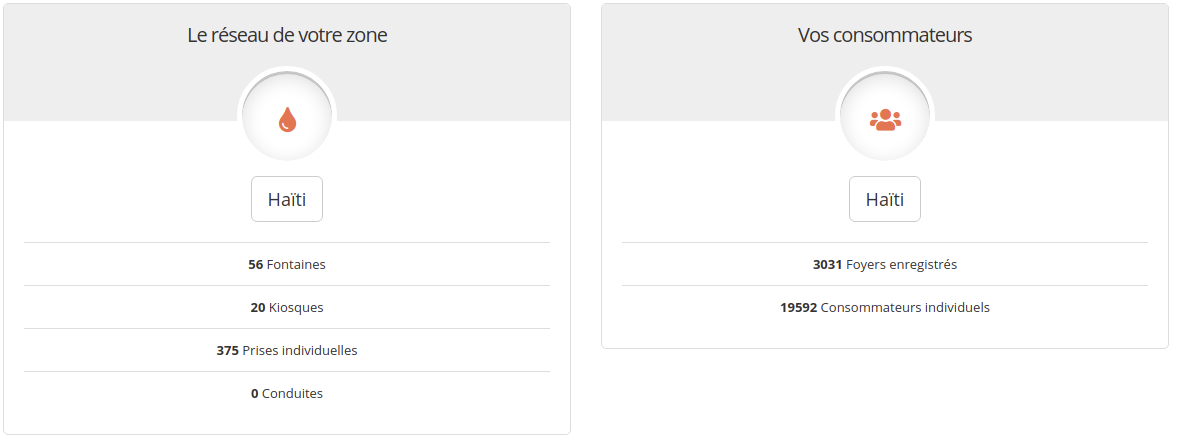
\includegraphics[width=1\textwidth]{images/dashboard}
					\caption{Module "Accueil"}
				\end{figure}
				
				
			\subsection*{Module "Réseau"}
				\label{sec:reseau}
				Dans ce module, l'utilisateur peut retrouver trois éléments différents (cf. figure \ref{fig:reseau}).
				
				\begin{description}
				\item[Schéma] Ce schéma représente la répartition des consommateurs selon leur genre ou le volume d'eau mensuel distribué dans chaque zone. L'utilisateur peut sélectionner le schéma à afficher grâce à une liste déroulante.
				\item[Résumé de zone] Ce résumé présente le nombre de consommateurs et de points d'eau présents ainsi que le volume d'eau distribué dans la zone attribuée à l'utilisateur.
				\item[Eléments du réseau] Ce tableau reprend tous les différents éléments du réseau. Dans cette partie, en fonction de ses privilèges, l'utilisateur peut ajouter, modifier ou supprimer des éléments du réseau. Il peut également trier ou rechercher les éléments du réseau, si nécessaire.
				\end{description}
				
				\begin{figure}[H]
					\centering
					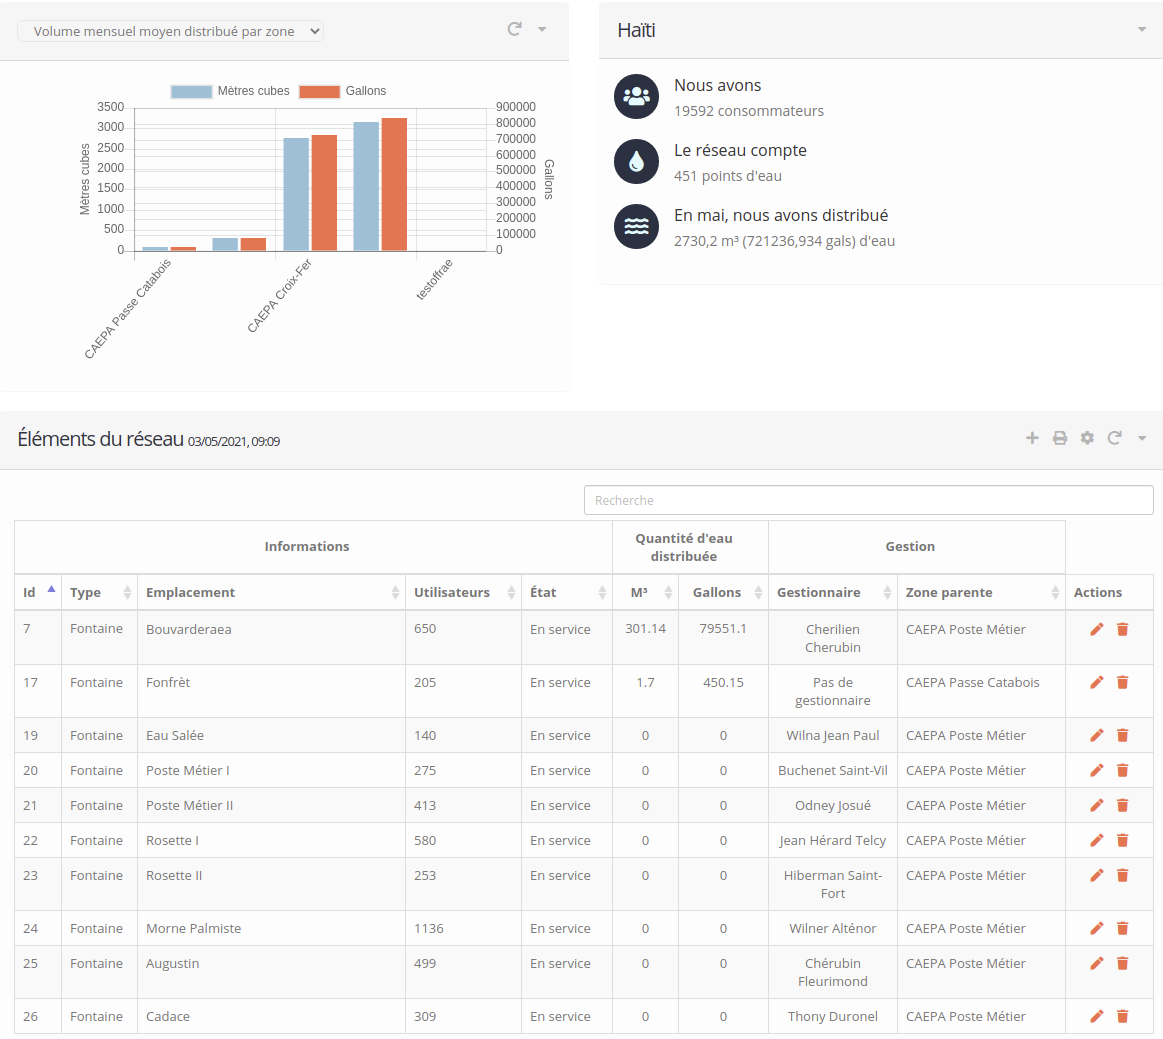
\includegraphics[width=1\textwidth]{images/water_elem}
					\caption{Module "Réseau"}
					\label{fig:reseau}
				\end{figure}
				
				
			\subsection*{Module "Carte"}
				Ce module comprend un tableau réduit des éléments du réseau ainsi qu'une carte interactive qui permet à l'utilisateur de voir où sont situés les différents éléments du réseau et de connaître ou d'encoder les coordonnées géographiques de ceux-ci (cf. figure \ref{carte}). Pour encoder ces coordonnées, l'utilisateur peut soit les entrer manuellement, soit utiliser la carte interactive prévue à cet effet. Comme dans le module décrit au point \ref{sec:reseau}, l'utilisateur peut ajouter, modifier ou supprimer des éléments du réseau.
			
				\begin{figure}[H]
					\centering
					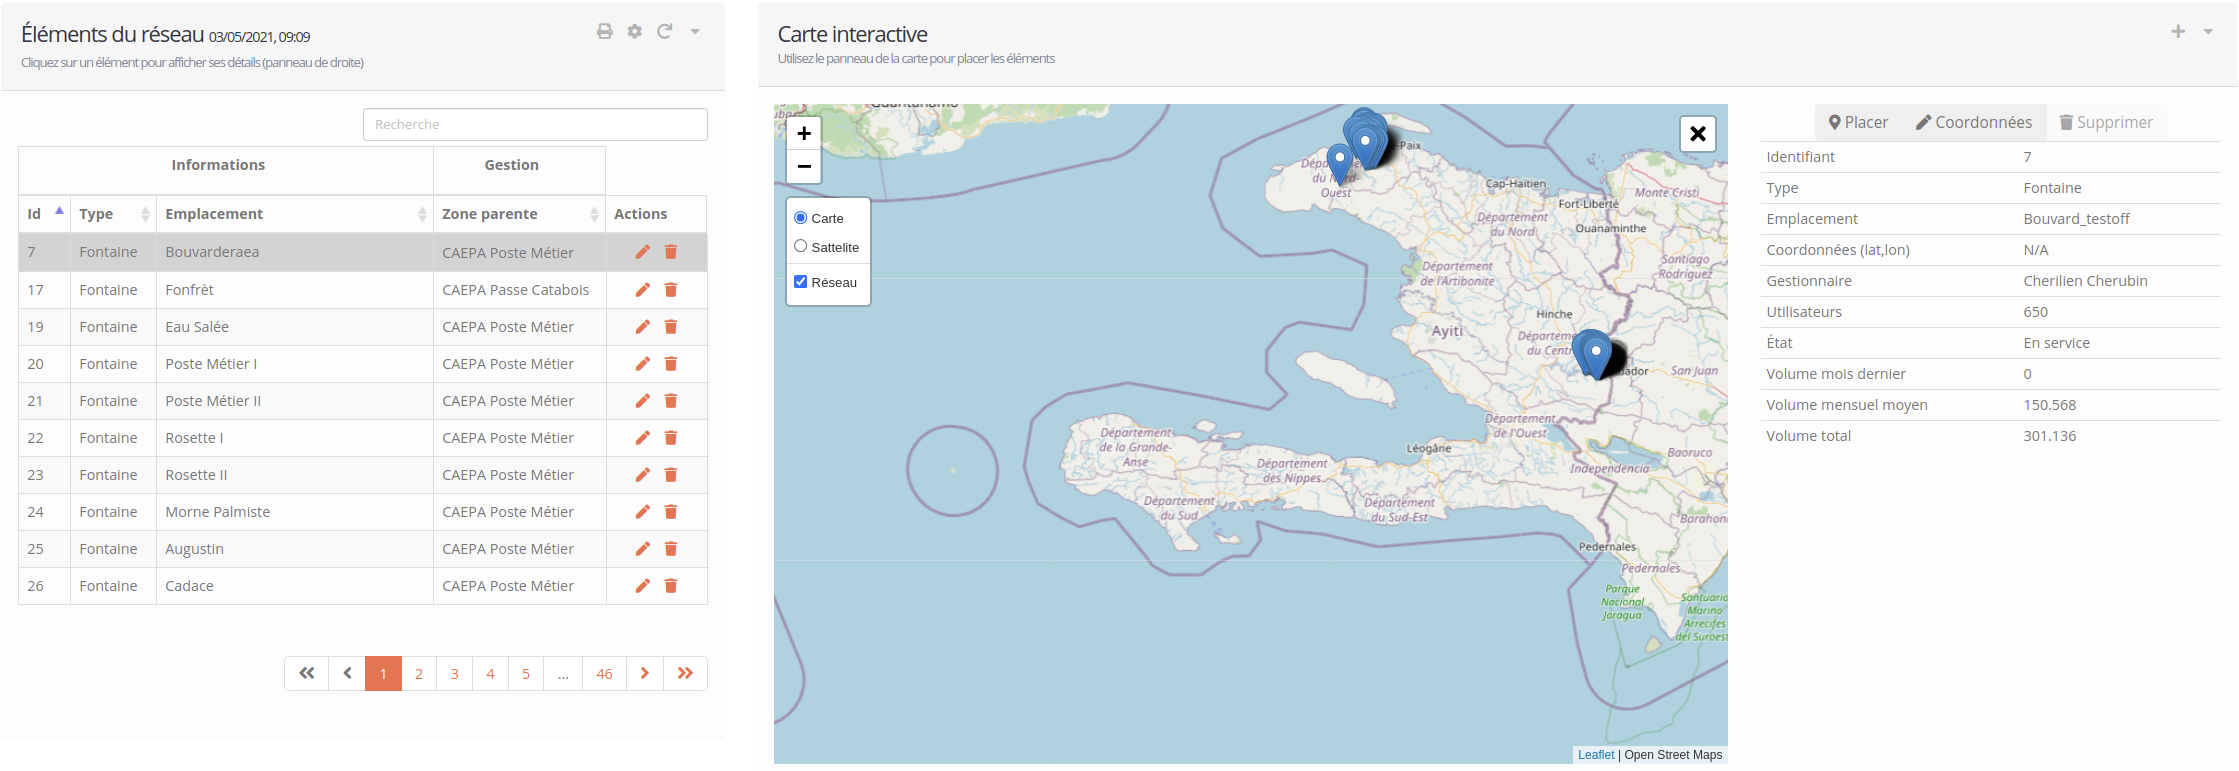
\includegraphics[width=1\textwidth]{images/map}
					\caption{Module "Carte"}
					\label{carte}
				\end{figure}
				
				\begin{figure}[H]
					\begin{subfigure}[b]{0.5\textwidth}
  						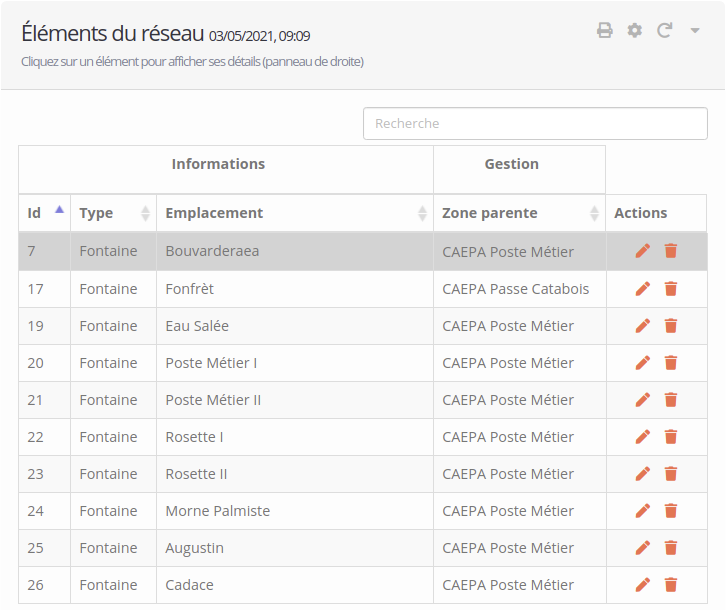
\includegraphics[width=1\linewidth]{images/map_tab1}
  						\caption{Tableau simplifié des éléments réseaux}
					\end{subfigure}%
					\begin{subfigure}[b]{0.5\textwidth}
  						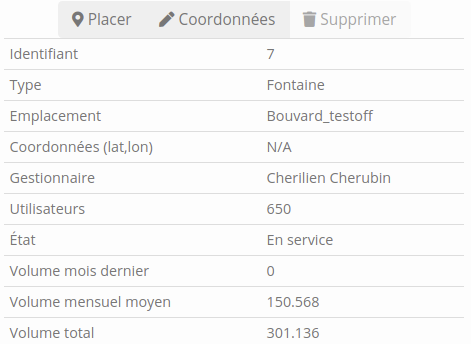
\includegraphics[width=1\linewidth]{images/map_tab2}
  						\caption{Détails de l'élément réseau}
					\end{subfigure}
				\end{figure}
				
				
			\subsection*{Module "Gestion de zone"}
				Ce module comprend trois tableaux permettant à l'utilisateur de gérer la zone qui lui est attribuée (cf. figure \ref{fig:zone}).
				\begin{description}
					\item[Zones] Le premier contient les différentes zones géographiques encodées dans le système. Cliquer sur un des éléments du tableau permet de filtrer les éléments des deux autres tableaux décrits plus bas afin de ne garder que les éléments de la zone concernée. Si l'utilisateur a les privilèges requis, ce tableau permet également d'ajouter, modifier ou supprimer une zone.
					\item[Gestionnaires] Le deuxième contient la liste de tous les gestionnaires. Cliquer sur un gestionnaire permet à l'utilisateur de filtrer les éléments réseaux qui sont gérés par ce premier. De nouveau, si l'utilisateur possède les privilèges requis, il pourra ajouter, modifier ou supprimer des gestionnaires.
					\item [Elements du réseau] Le dernier tableau est identique à celui de la section \ref{sec:reseau}.
				\end{description}
				
				\begin{figure}[H]
					\centering
					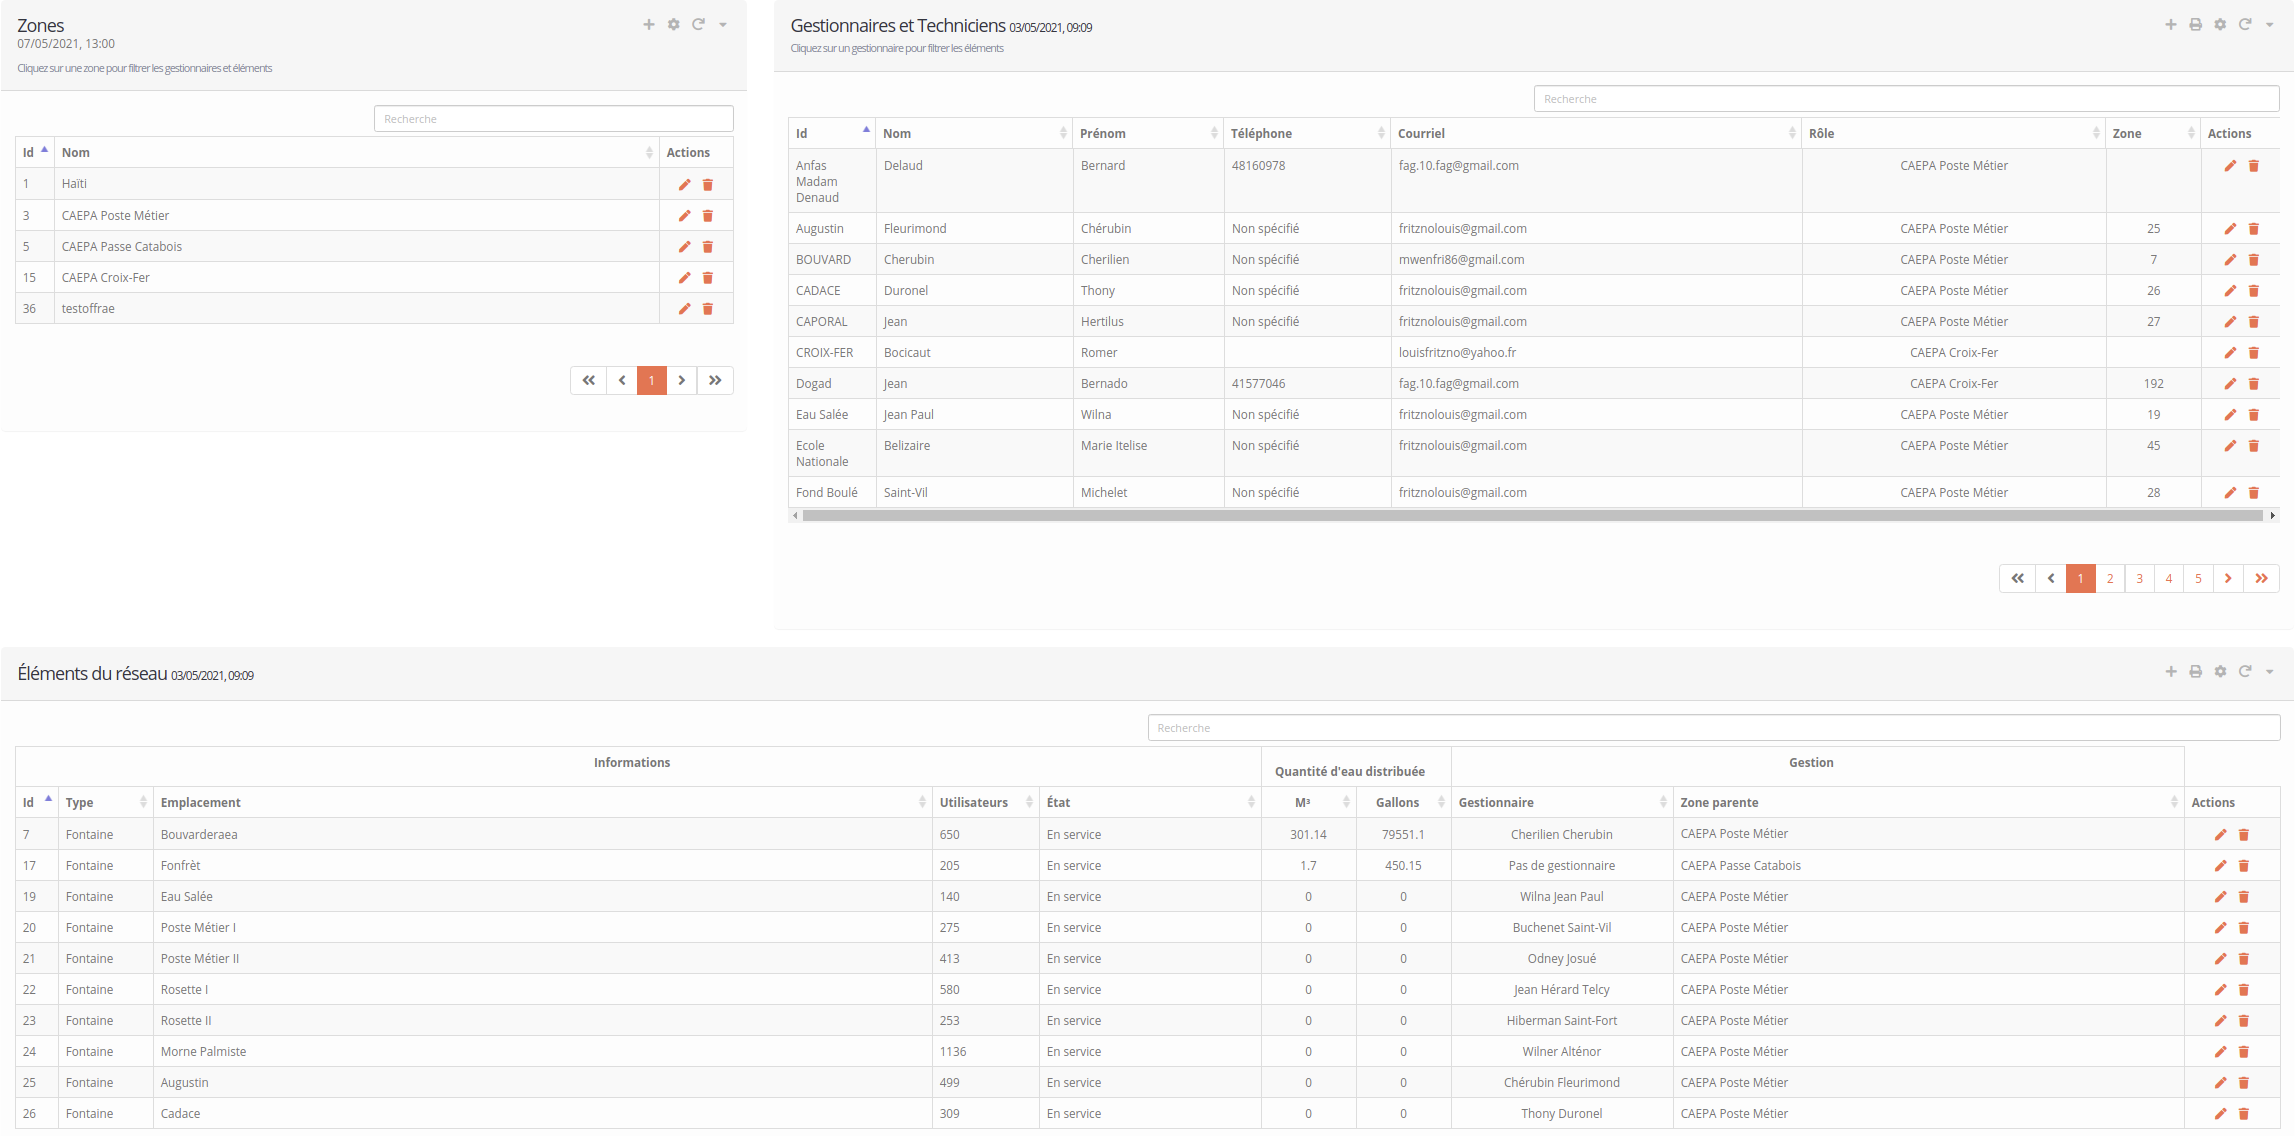
\includegraphics[width=1\textwidth]{images/gestion}
					\caption{Module "Gestion de zone"}
					\label{fig:zone}
				\end{figure}
			
				
				\begin{figure}[H]
					\begin{subfigure}[b]{0.3\textwidth}
  						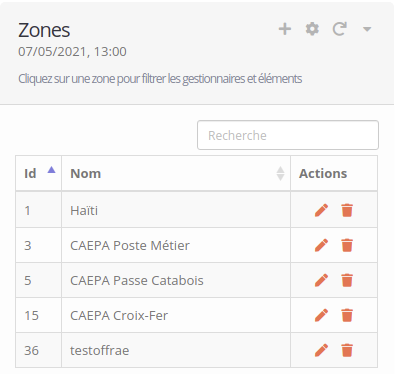
\includegraphics[width=1\linewidth]{images/gestion_tab1}
  						\caption{Tableau des zones}
					\end{subfigure}%
					\begin{subfigure}[b]{0.7\textwidth}
  						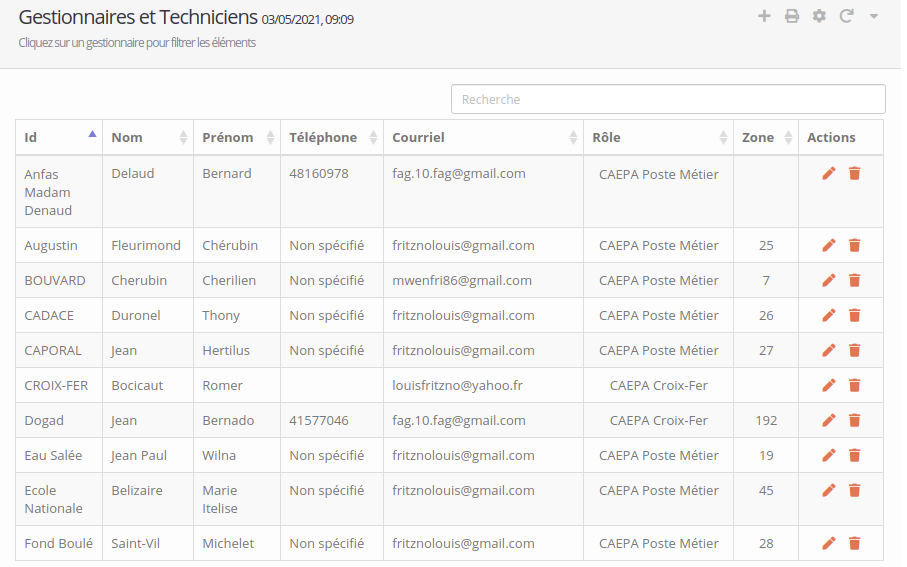
\includegraphics[width=1\linewidth]{images/gestion_tab2}
  						\caption{Tableau des gestionnaires}
					\end{subfigure}
				\end{figure}
			
			
			\subsection*{Module "Historique"}
			\label{sec:historique}
				Ce module contient les actions ayant été effectuées par des gestionnaires de fontaines. Ces actions doivent être traitées (validées ou refusées) par un gestionnaire plus haut placé. On peut y retrouver deux tableaux (cf. figure \ref{fig:historique}).
				\begin{description}
					\item[A valider] Ce tableau reprend les éléments en attente de traitement: le gestionnaire de zones peut valider ou refuser l'action encodée.
					\item[Historique] Ce tableau reprend les éléments qui ont été validés ou refusés dans les trois dernières semaines. Il s'agit de l'historique récent des dernières modifications.
				\end{description}
				\begin{figure}[H]
					\centering
					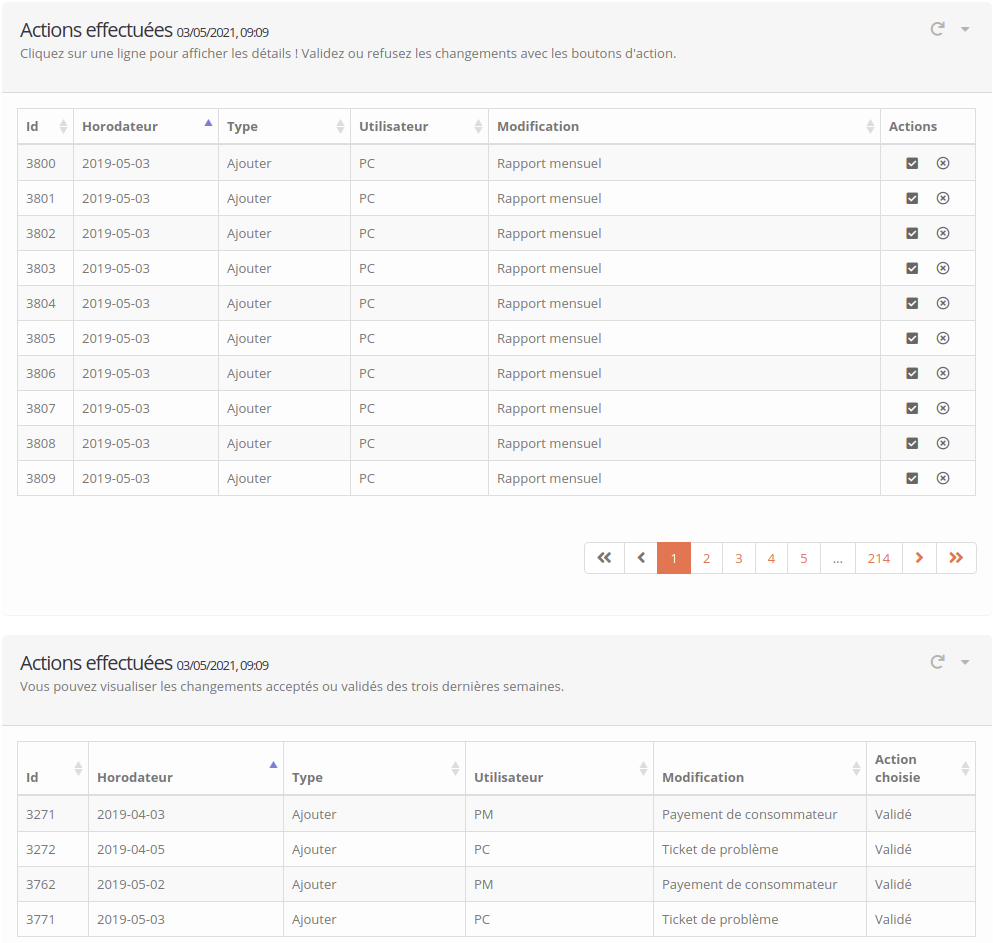
\includegraphics[width=0.9\textwidth]{images/logs}
					\caption{Module "Historique"}
					\label{fig:historique}
				\end{figure}
				
			
			\subsection*{Module "Rapports"}
				Dans ce module, l'utilisateur peut signaler les différents problèmes qu'il rencontre avec les infrastructures de distribution d'eau potable. Le problème signalé, l'utilisateur peut consulter, modifier ou supprimer son signalement. Si ses privilèges sont suffisamment élevés, il pourra également gérer les signalements d'autres utilisateurs (cf. figure \ref{fig:rapport}).
				
				C'est également ici que l'utilisateur va pouvoir encoder les rapports mensuels. Si jamais la connexion au serveur n'est pas disponible, il peut sauvegarder le formulaire avec les données qu'il a encodées afin de l'envoyer plus tard lorsque la connexion sera rétablie.
				
				\begin{figure}[H]
					\centering
					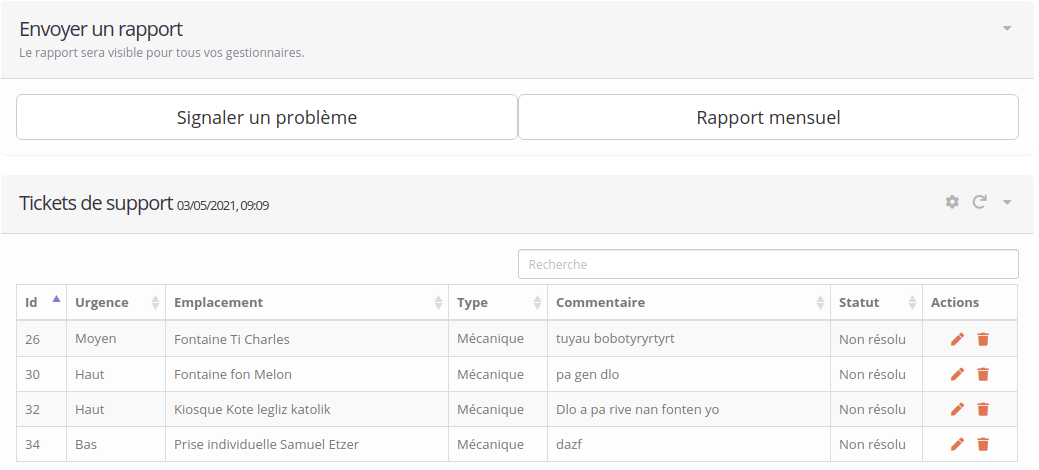
\includegraphics[width=1\textwidth]{images/report}
					\caption{Module rapport}
					\label{fig:rapport}
				\end{figure}
			
			
			\subsection*{Module "Consommateurs"}
				Dans ce module, l'utilisateur retrouve trois parties différentes (cf. figure \ref{fig:consumer}).
				\begin{description}
					\item[Schéma] Ce schéma est celui de la section \ref{sec:reseau}.
					\item[Résumé de zone] Cette partie présente un résumé de la zone attribuée à l'utilisateur (nombre de foyers consommant de l'eau, nombre de consommateurs, nombre de foyers n'ayant pas payé leur facture).
					\item[Consommateurs] Ce tableau reprend tous les consommateurs appartenant à la zone attribuée à l'utilisateur. Celui-ci peut ajouter, modifier ou supprimer des consommateurs. Il peut également consulter tous leurs détails.
				\end{description}
				

				
				\begin{figure}[H]
					\centering
					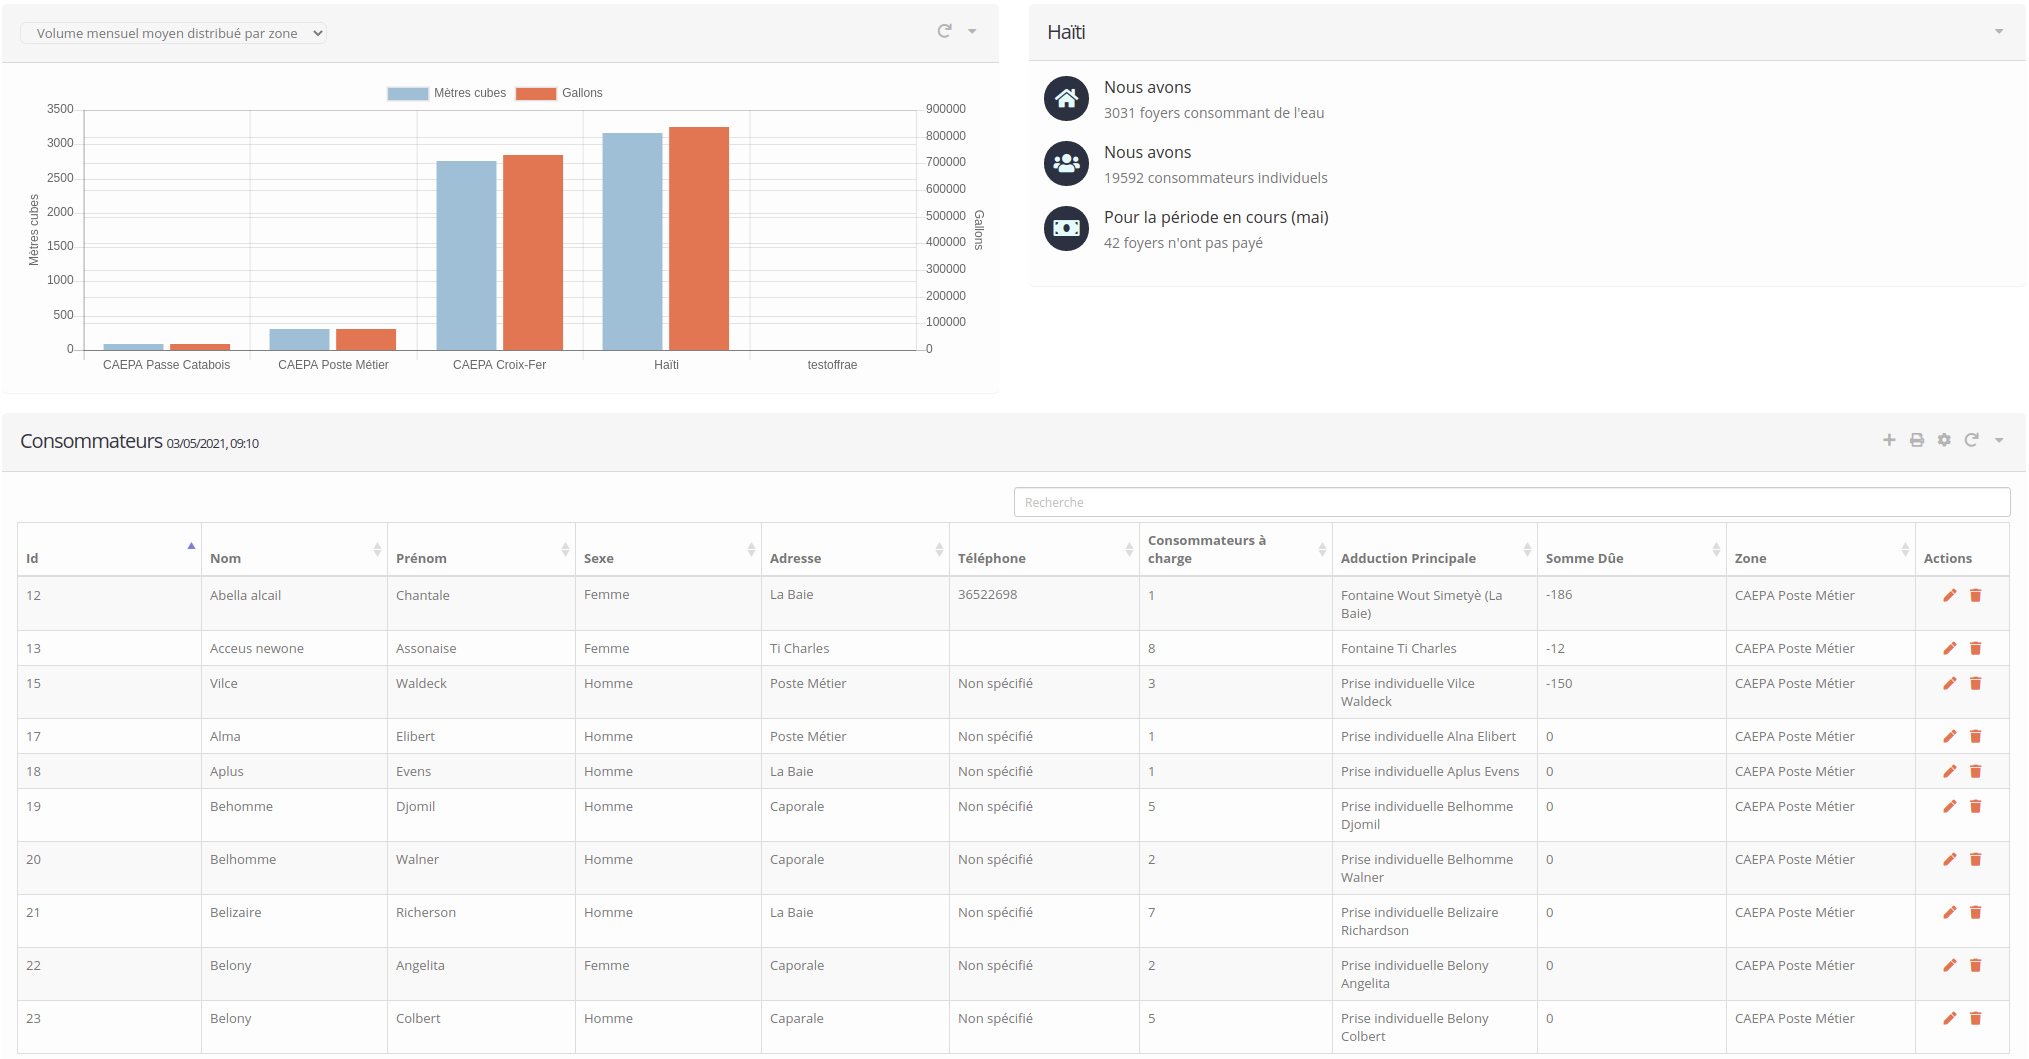
\includegraphics[width=1\textwidth]{images/consumer}
					\caption{Module "Consommateurs"}
					\label{fig:consumer}
				\end{figure}
				
				\begin{figure}[H]
					\centering
					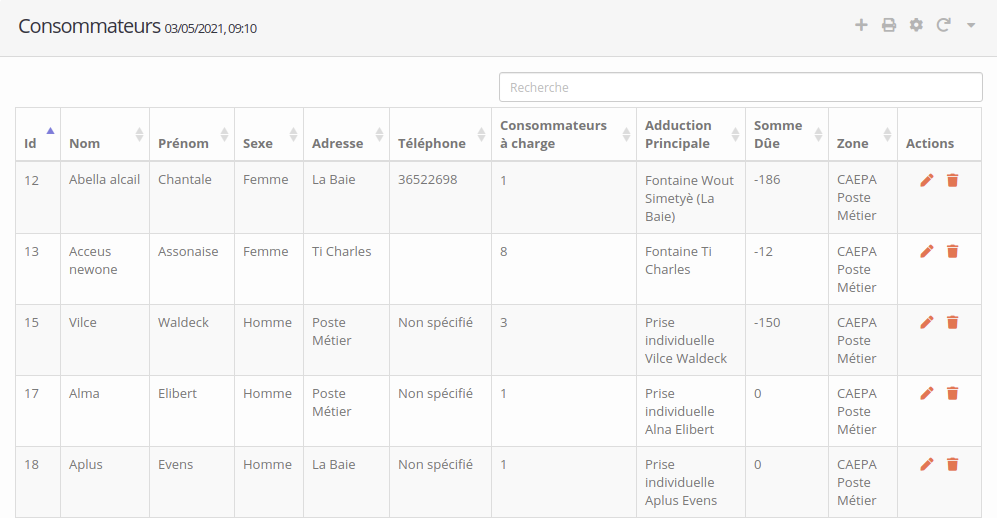
\includegraphics[width=1\textwidth]{images/consumer_tab1}
					\caption{Tableau des consommateurs}
				\end{figure}
			

			\subsection*{Module "Finances"}
				Dans ce module, l'utilisateur a accès à quatre tableaux différents qui lui permettent de gérer les finances de ses consommateurs. Celui-ci pourra ajouter, modifier ou supprimer des informations dans les différents tableaux en fonction de son niveau de privilèges (cf. figure \ref{fig:finance1} et \ref{fig:finance2}).
				
				\begin{description}
					\item[Zones] Ce tableau contient les zones attribuées à l'utilisateur. Le fait de sélectionner une zone permet à l'utilisateur de filtrer les consommateurs.
					\item[Consommateurs] Ce tableau reprend les consommateurs appartenant à la zone attribuée à l'utilisateur. Le fait de sélectionner un consommateur permet de faire apparaître les deux tableaux suivants.
					\item[Détails] Ce tableau reprend les coordonnées du consommateur sélectionné ainsi que la somme due par celui-ci. Il n'est pas possible de modifier des données dans ce tableau.
					\item[Paiements] Ce tableau reprend tous les paiements effectués par le consommateur sélectionné. L'utilisateur peut ajouter, modifier ou supprimer les paiements du consommateur séléctionné.
				\end{description}
				
				\begin{figure}[H]
					\centering
					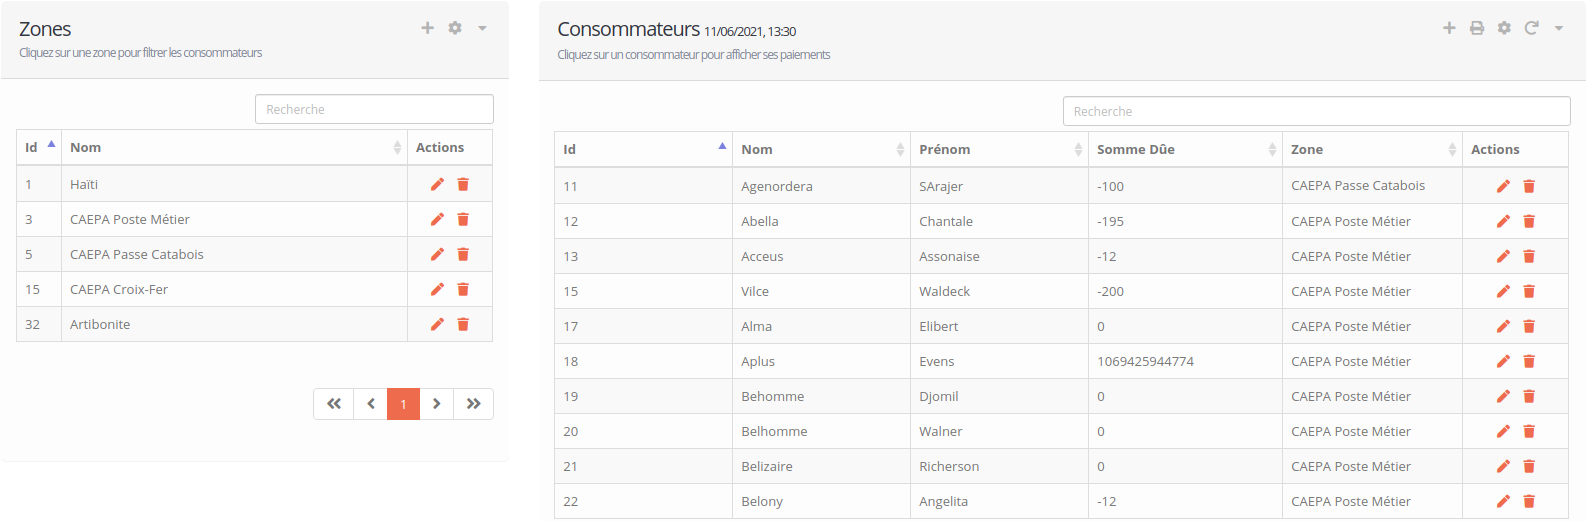
\includegraphics[width=1\textwidth]{images/finances1}
					\caption{Module "Finances" partie 1}
					\label{fig:finance1}
				\end{figure}
				
				\begin{figure}[H]
					\centering
					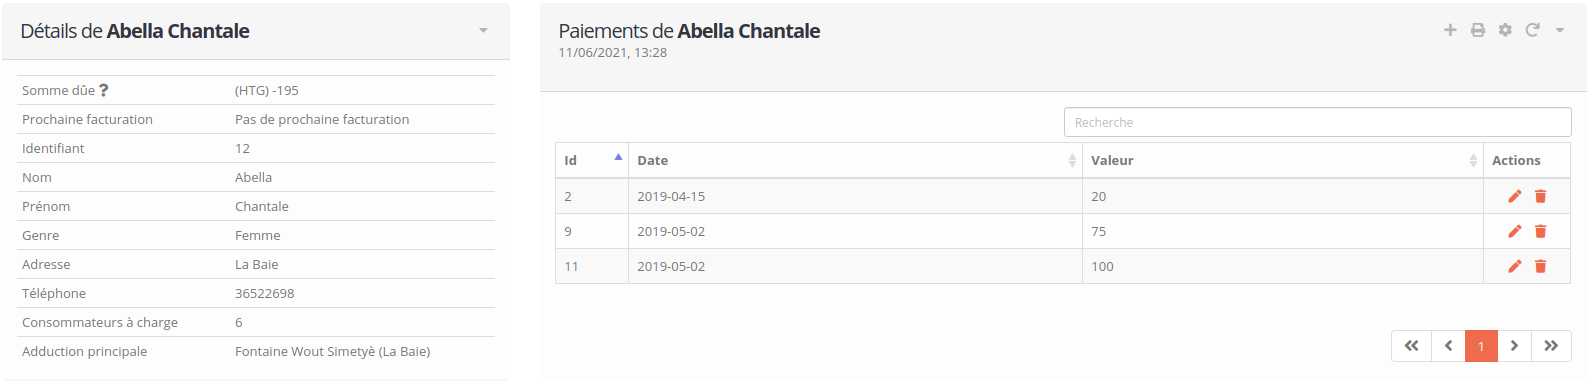
\includegraphics[width=1\textwidth]{images/finances2}
					\caption{Module "Finances" partie 2}
					\label{fig:finance2}
				\end{figure}
				
				
		\section{Problèmes réseaux}
			L'application HaïtiWater est une application web classique. Cela signifie que pour fonctionner, il faut qu'il y ait nécessairement une connexion au serveur. Or, en Haïti, cette connexion n'est pas très stable en ville et peut aller jusqu'à être inexistante dans les zones les plus rurales. 
			
			Ces problèmes de connexion rendent difficile l'utilisation sereine de l'application sur le terrain. Pour pallier ce problème, il a été décidé de faire évoluer l'application web existante de manière à fonctionner lorsque la connexion au serveur est absente.
				
			Au vu de sa nature, une application web nécessite une connexion pour fonctionner. Il a donc fallu étudier les différentes options qui pourraient permettre à l'application de fonctionner hors-ligne. Parmi ces options,  les deux retenues étaient la création d'une \textbf{application mobile} séparée de l'application web, ou la transformation de l'application web existante en \textbf{\gls{pwa}}. 
				
			
			
			
		
			
			
%------------------------------------------------------------------------------------------

	\chapter{Organisation}
		Etant le seul étudiant à réaliser ce mémoire, il n'a pas été nécessaire d'utiliser des outils de planification collaboratif. Cette section contiendra surtout la planification des différentes tâches à accomplir permettant l'évolution de l'application ainsi que l'écriture de ce mémoire. Celles-ci ont été mises en place grâce aux discussions avec mes deux promoteurs. 

		\section{Approche de travail}
			La première étape de  mon mémoire a été de mettre en avant les différentes fonctionnalités à implémenter afin d'ajouter de la plus-value au projet existant, l'idée de base étant de rendre l'application fonctionnelle hors-ligne.	
			
			Nous avons étudié la question avec mes deux promoteurs et Nahomie, une étudiante venue de Haïti. Cette dernière nous a apporté son expertise afin de séléctionner les fonctionnalités qui pourraient apporter une réelle plus-value au projet et de prioriser l'implémentation de celles-ci.
		

			\subsection*{Planification}
				\label{sec:planification}
				
				\paragraph*{Mensuelle}
				D'abord, il a fallu réaliser un plan général de la réalisation du mémoire, mettre en avant les modules sur lesquels il fallait travailler en priorité et les différentes fonctionnalités à implémenter. Une échéance importante était le test de la nouvelle version de l'application par des utilisateurs à partir de février afin d'obtenir un feedback concret et pertinent.
								
				\paragraph*{Hebdomadaire} 
				Une réunion était prévue toutes les semaines en alternance avec mes deux promoteurs. Ces réunions permettaient de leur montrer l'état d'avancement du développement de l'application et d'avoir un feedback extérieur. Elles ont toutes eu lieu en appel vidéo via l'application Microsoft Teams. En effet, à cause de la conjoncture liée à la crise sanitaire mondiale, il était impossible de tenir nos réunions en présentiel.
				
				\paragraph*{Quotidienne}
				Pour gérer l'organisation de mon travail, une liste de tâches était maintenue. Cette liste était modifiée tous les jours en fonction du travail effectué. Les plus importantes étaient maintenues en haut de la liste afin de les prioriser. 
				
				Le plan n'a malheureusement pas pu être entièrement respecté pour différentes raisons:
				\begin{itemize}
					\item La technologie employée (voir section \ref{sec:choix_tech}) étant encore assez récente, les sources d'informations et d'aides sur internet sont encore peu fournies. Du retard a donc été pris lors du développement de certaines fonctionnalités complexes,
					\item L'installation du serveur en Haïti a pris plus de temps que prévu; il a donc fallu retarder le test de la nouvelle version de l'application par des utilisateurs,
					\item Le bal des mesures sanitaires à relativement influencé ma motivation et mon implication dans la réalisation de mon travail.
				\end{itemize}				
				
				Malgré le retard accumulé, il a tout de même été possible de terminer le projet dans les temps.
				
				
				
		\section{Méthodologie}
			Même en travaillant seul, une bonne méthodologie de travail permet de garantir l'avancement régulier du projet. Elle permet de transformer efficacement les différents besoins en fonctionnalités implémentées.
			

			\subsection*{Agile}
				La méthodologie agile permet une réponse plus flexible au changement. Plûtot que de planifier tout le projet directement, il est conseillé de développer par petit incrément finalisé à chaque itération. 
				
				Cette méthode a permis l'évolution du projet en fonction des différents feedback reçus, ce qui n'aurait pas été possible avec une approche waterfall plus séquentielle.
				
				\paragraph*{Feature Driven Development} Cette méthode s'attarde sur la création la création d'une liste de fonctionnalités et de leur production. Ces différentes fonctionnalités ont été déterminées par mes deux promoteurs, l'étudiante haïtienne.
				
				\paragraph*{Itérations} Dans le cadre d'une méthodologie agile, les itérations sont de courtes durées. Lors de ce mémoire, les itérations duraient deux semaines. Cela permettait d'avoir un feedback de la part des deux promoteurs que je voyais en alternance une semaine sur deux. Les avantages des itérations courtes sont la détection rapide des défauts présents ainsi que leur correction. 
			
			
%---------------------------------------------------------------------------------------------

	\chapter{Analyse des besoins}
		\label{sec:analyse_besoins}
		Cette phase est très importante. En effet, nous, mes deux promoteurs, l'étudiante de Haïti et moi-même, avons choisi quelle technologie était la plus adaptée afin de faire évoluer l'application existante de la meilleure façon possible. Nous avons également déterminé toutes les fonctionnalités à implémenter et leur ordre de priorité.
		
		Avec l'aide de l'étudiante haïtienne et les bons conseils de mes promoteurs, j'ai realisé une analyse de Moscow décrite dans la section \ref{sec:besoins_fonctionnels}. Cette méthode permet de prioriser les tâches d'un projet en fonction de leur criticité, c'est-à-dire du niveau d'impact de la tâche sur la réalisation du projet.
		Cette analyse de \gls{moscow} est assez représentative de la direction que devait prendre le projet et représente les différentes tâches à accomplir de manière fidèle.


		\section{Besoins fonctionnels}
			\label{sec:besoins_fonctionnels}	
				
			\begin{figure}[H]
				\centering
				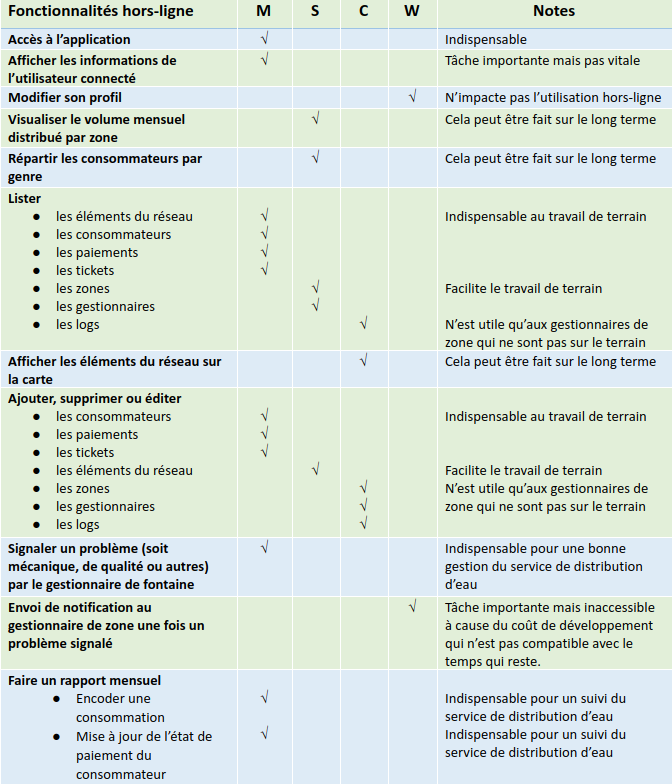
\includegraphics[width=1\textwidth]{images/moscow}
				\caption{Analyse de Moscow des fonctionnalités hors-ligne}
				\label{fig:moscow}
			\end{figure}
			
			Les besoins fonctionnels répondent aux points précis à implémenter et représentent toutes les tâches à accomplir pour que le projet soit réussi. Dans le tableau \ref{fig:moscow}, les lettres ont la signification suivante: 
			\begin{itemize}
				\item \textbf{M} signifie "Must have", le projet serait un échec si l'application ne possédait pas cette fonctionnalité à la fin du développement,
				\item \textbf{S} signifie "Should have", cette fonctionnalité doit être développée dans la mesure du possible. Ces tâches sont importantes mais pas vitales,
				\item \textbf{C} signifie "Could have", cette fonctionnalité peut être développée si cela n'affecte pas les autres tâches plus importantes. Ce sont des tâches de confort qui peuvent être effectuées si le temps le permet et que les tâches des deux catégories précédentes ont été réalisées,
				\item \textbf{W} signifie "Won't have but would like", ce qui ne sera pas développé cette fois, mais plus tard. Réaliser ces tâches est un luxe théoriquement imopssible.
			\end{itemize}

			
			Toutes les tâches de type \textbf{M}, \textbf{S} et \textbf{C} ont été réalisées durant ce projet. Seules les tâches \textbf{W} n'ont pas été implémentées.
			
			Lors de l'analyse des besoins, nous avons bien entendu repris l'analyse faite par les anciens mémorants \cite{ref:haitiwater}. Ils proposaient trois types différents d'accès à l'application et aux données lorsque la connexion au serveur n'est pas disponible. Les trois options proposées sont les suivantes. 
			
			\begin{description}
				\item[Accès aux formulaires] Avec cette solution, l'utilisateur aurait un accès permanent aux différents formulaires d'ajout de données. Celui-ci pourrait pré-remplir les formulaires et les sauvegarder dans le cache du navigateur afin de les envoyer plus tard dans le cas où la connexion n'était pas disponible immédiatement. Cette solution est déjà partiellement mise en place dans l'application de base. Il est en effet déjà possible de pré-remplir son rapport mensuel et de le sauvegarder pour plus tard.
				\item[Accès statique aux données] Cette solution requiert l'accès à une copie simplifiée de la base de données sur l'appareil de l'utilisateur sans possibilité de modification. Cela permettrait aux utilisateurs de consulter les données hors-ligne mais pas d'en entrer de nouvelles. L'avantage de cette solution est que la synchronisation des tables est très simple et qu'il n'y a pas de problèmes d'inconsistances des données qui peuvent arriver lorsque deux utilisateurs modifient la même donnée en étant hors-ligne.
				\item[Accès complet aux données] Cette solution permettrait aux utilisateurs de consulter, ajouter, modifier et supprimer des données de la base de données. Ainsi, même en cas de perte de connexion au serveur, l'utilisateur pourrait continuer à réaliser ses tâches sans le moindre souci. Cette solution est la plus compliquée à mettre en place à cause de la synchronisation des différentes versions des données. En effet, si deux utilisateurs modifient en même temps les mêmes données en étant hors-ligne, il faudrait pouvoir déterminer quelles modifications conserver sans créer d'inconsistance.  
			\end{description}
			
			L'option choisie est l'accès complet aux données. C'est la seule solution qui permettrait vraiment à l'application d'être utilisée de manière intensive sur le terrain. C'est également l'option la plus intéressante à mettre en place du point de vue technique.
			
			
			\subsection*{Affichage des pages}
				Une partie importante des besoins est bien évidemment l'accès aux différentes pages de l'application lorsque la connexion au serveur n'est plus disponible. 
				
				C'était la partie prioritaire du projet; sans cette fonctionnalité, il aurait été impossible pour l'utilisateur d'accèder aux différentes données. Les premières pages concernées par cette évolution ont été celles utiles aux gestionnaires de fontaines qui sont le plus souvent sur le terrain.
				Les différents points du tableau \ref{fig:moscow} concernés par cette partie sont:
				\begin{itemize}[noitemsep]
					\item Accéder à l'application,
					\item Afficher les informations de l'utilisateur connecté,
					\item Visualiser le volume mensuel distribué par zone,
					\item Répartir les consommateurs par genre.
				\end{itemize}
				
				Nous constatons que les deux premiers points sont bien placés dans la catégorie "Must have". Les deux derniers sont dans le "Should have". En effet, ces fonctionnalités ne sont que des schémas qui s'affichent sur certaines pages et ceux-ci ne sont pas essentiels.
				
				
			\subsection*{Accès aux données}
				La deuxième partie importante des besoins fonctionnels est d'avoir accès aux données de la base de données même lorsque la connexion au serveur n'est pas disponible. En effet, le simple accès aux pages hors-ligne sans pouvoir consulter de données n'a que peu d'intéret.
			Dans le tableau \ref{fig:moscow}, cela est représenté par les points suivants :
				\begin{itemize}[noitemsep]
					\item Lister les éléments du réseau,
					\item Lister les consommateurs,
					\item Lister les paiements,
					\item Lister les tickets,
					\item Lister les zones,
					\item Lister les gestionnaires,
					\item Lister les logs.
				\end{itemize}
				
				Les quatre premiers points sont dans la catégorie "Must have". Ceux-ci représentent les données qui seront utilisées en permanence par les utilisateurs sur le terrain, les gestionnaires de fontaines. Ce sont donc les données qu'il faut prioritairement avoir dans l'application hors-ligne.
				
				Les trois derniers sont dans la catégorie "Should have" et "Could have". Ceux-ci sont surtout utiles pour les gestionnaires de zones qui seront assez peu sur le terrain. Malgré tout, il reste intéressant de pouvoir accèder à ces données même lorsque la connexion au serveur n'est pas disponible dans le cas où un gestionnaire devrait se déplacer sur le terrain.
				
				Un dernier point non listé est d'afficher les éléments du réseau de distribution d'eau sur une carte interactive même lorsque l'on a pas de connexion au serveur. Ce point a été mis dans les "Could have"; l'usage de la carte en mode hors-ligne est une fonction qui prendrait beaucoup d'espace sur un appareil mobile et cette fonctionnalité n'est pas essentielle à un usage sur le terrain.

			\subsection*{Modifications des données}
				\label{sec:gest_donnee}
				La dernière partie mais non la moindre consiste à gérer l'envoi des données lorsque la connexion au serveur n'est pas disponible. Cela permettrait aux utilisateurs de complètement se passer de la solution crayon et papier.
				Dans le tableau \ref{fig:moscow}, cette partie est représentée par les points suivants:
				\begin{itemize}[noitemsep]
					\item Ajouter, éditer ou supprimer:
					\begin{itemize}[noitemsep]
						\item Les consommateurs,
						\item Les paiements,
						\item Les tickets,
						\item Les zones,
						\item Les gestionnaires,
						\item Les logs,
					\end{itemize}
					\item Signaler un problème par le gestionnaire de fontaines,
					\item Faire un rapport mensuel.
				\end{itemize}
				
				La plupart des points sont situés dans la partie "Must have". Ces fonctionnalités sont effectivement essentielles au bon fonctionnement de l'application hors-ligne. Par contre, la modification des éléments du réseau, des zones, des gestionnaires et des tickets sont dans les catégories "Should have" and "Could have", ces données étant surtout utilisées par les gestionnaires de zones qui ne vont que peu sur le terrain.			

		\section{Besoins non-fonctionnels}
			Les besoins non-fonctionnels sont soit des besoins optionnels, soit des besoins liés à l'implémentation et à l'interopérabilité générale. C'est en réalisant ces besoins non-fonctionnels qu'est obtenu un système fiable et qualitatif.
					
			\subsection*{Multi-plateforme}
			\label{sec:multi}
				C'est dans le cadre de la suite d'un mémoire universitaire que s'inscrit mon projet. A terme, la nouvelle version de l'application sera déployée et maintenue par une équipe de développeurs en Haïti.
				
				Cependant, un problème persiste; le temps et le budget qui seront alloués à la suite de ce projet ne sont pas encore connus. Par contre, il est primordial que l'application puisse tourner sur un maximum d'appareils différents. Les choix technologiques décrits dans la section \ref{sec:choix_tech} ont donc été pris en tenant compte du faite que l'application doit pouvoir tourner sur tout type de configuration.
				
			\subsection*{Technologies simples et populaires}
				Comme précisé précédemment, nous ne connaissons pas encore l'équipe de développeurs qui va reprendre le projet. Il a donc fallu continuer à utiliser des technologies qui sont assez rapides à apprendre et accessibles à tous, cela afin de faciliter la maintenance et l'évolutivité de l'application lorsque celle-ci sera déployée en Haïti.	
				
				De plus, il faudra également fournir une documentation complète et détaillée dans le but d'aider ces futurs développeurs lorsqu'ils devront reprendre l'application.
				
		\section{Structure des données hors-ligne}
			\label{sec:data}
			Pour que l'utilisateur puisse accèder aux données en étant hors-ligne, il faut bien évidemment que celles-ci soient stockées sur l'appareil. Pour ce faire, il a fallu trouver une solution peu gourmande en stockage, accessible rapidement en lecture et permettant la modification des données. Deux solutions ont alors été envisagées.
			\begin{description}
				\item[JSON] Stocker les réponses au format \gls{json} telles qu'envoyées par le serveur dans le cache du navigateur. L'avantage de cette solution est qu'il est très rapide de récupérer les données à afficher sur la page lors du chargement de celle-ci, ces données étant stockées telles qu'utilisée par le navigateur. Cette solution est également très facile à mettre en place. Si notre choix s'était porté sur l'accès statique aux données, décrit dans la section \ref{sec:besoins_fonctionnels}, cette solution aurait été suffisante. Mais comme il faut pouvoir modifier les données, cette solution n'est pas la plus adaptée: il faudrait mettre le JSON en mémoire, le modifier et ensuite réecrire tout le nouveau \gls{json} dans le cache à chaque modification de données.
				\item[DB] Utiliser un système de gestion des données intégré au navigateur. Cette option a pour avantage d'avoir un système complet de gestion de données. Les données enregistrées dans le navigateur, il est très facile de lancer des requêtes (consulter, ajouter, modifier, supprimer) sur celles-ci. Par contre, l'inconvénient est que lors de la synchronisation des différentes tables dans le navigateur, l'appareil doit fournir un travail supplémentaire.
			\end{description}
				
			La solution retenue est la seconde. En effet, elle se montre plus optimal dans la gestion des données stockées localement (consulter, ajouter, modifier, supprimer).
			
			



%------------------------------------------------------------------------------------------------------------
	\chapter{Implémentation}

		\section{Application de base}
			Dans cette section, un résumé de l'application HaïtiWater créée précédemment sera présenté. Pour de plus amples informations sur les raisons des choix technologiques suivants et les détails de leur implémentation, le document \cite{ref:haitiwater} est en consultation libre.
			
			\subsection*{Backend}
				L'application HaïtiWater est une application web propulsée par le langage Python. C'est ce langage qui a été choisi pour le backend grâce à sa popularité et sa facilité d'apprentissage. Il existe énormément de librairies logicielles et de documentations sur internet.
				
				Vu la taille du projet, un \gls{framework} a dû être utilisé, l'organisation et la structure du framework permettant une productivité plus élevée qu'un développement sans \gls{framework} et facilitant la maintenance grâce une bonne organisation du code source. Le choix s'est porté sur \Gls{django} principalement pour ses outils de gestion de base de données particulièrement efficaces pour les données géographiques.	
			
				Le \gls{sgbd} utilisé pour l'application est \gls{postgres}. Ce dernier a été choisi pour deux raisons:
				\begin{itemize}
					\item \gls{postgres} est le système recommandé par \Gls{django}, celui-ci s'adaptant le mieux à l'\gls{orm2}. C'est \Gls{django} qui va se charger d'effectuer la connexion avec la base de données et qui va se charger d'y envoyer toutes les requêtes,
					\item dispose de l'extension \gls{postgis} permettant de traiter facilement les données géographiques.
				\end{itemize}			
				
				\Gls{django} utilise une architecture modulaire facilitant l'évolution et la maintenance de l'application. La figure \ref{fig:modules} représente les relations entre les différents modules tel que présenté dans le mémoire de la première version de l'application \cite{ref:haitiwater}.
				
				\begin{figure}[H]
					\centering
					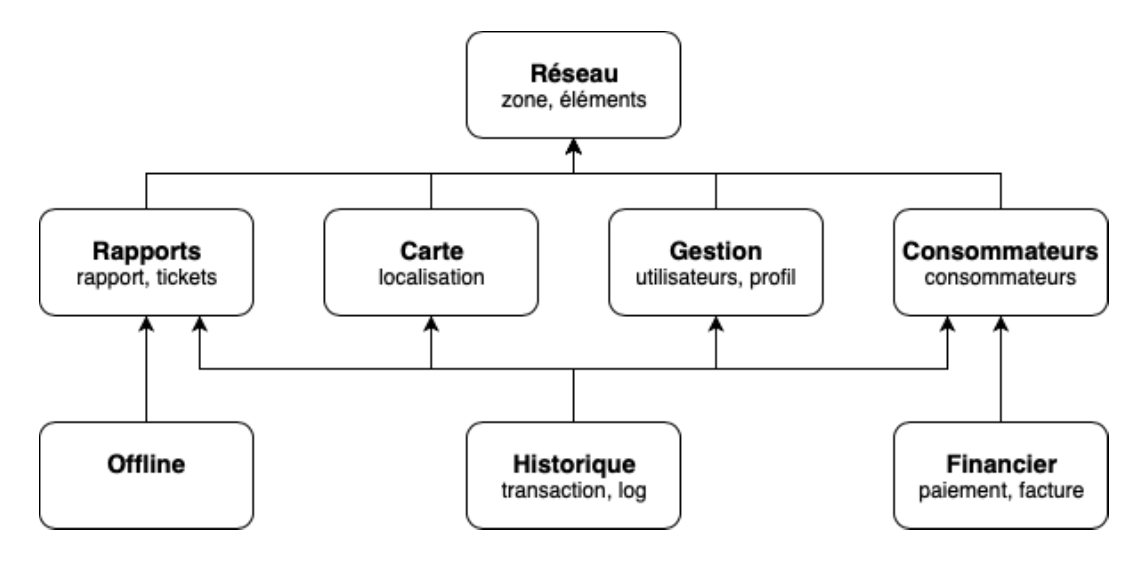
\includegraphics[width=1\textwidth]{images/modules}
					\caption{Relations entre les modules de l'application HaïtiWater}
					\label{fig:modules}
				\end{figure}						
				
				Le serveur possède également une \gls{api} qui lie l'\gls{orm} de \Gls{django} et les requêtes du client pour récupérer des données dans la base de données. Les requêtes concernant une page à afficher et celles concernant les données sont donc séparées. Cela facilite la récupération des données par les différentes bibliothèques du frontend et, en cas de création d'une autre application, permet de continuer à récupérer les informations sur le serveur.
						
			\subsection*{Frontend}
				Pour le design du frontend, la librairie bootstrap a été utilisée. Elle permet l'agencement de et la personnalisation de l'interface graphique au moyen de blocs. La raison de son utilisation est qu'il s'agit d'une bibliothèque très connue et utilisée, donc facile à apprendre.
				
				Pour l'affichage des données, deux autres bibliothèques ont été employées. La première, "datatable.js", permet l'affichage des données sous forme de table, leur recherche et le lancement de leur modification. La seconde, "chart.JS", permet l'affichage des données sous forme de graphiques. Toutes les données sont récupérées par les blibliothèques via l'\gls{api} du serveur.
				
			\subsection*{Client}
				L'application utilise la mise en cache afin d'éviter les télechargements répétitifs des mêmes fichiers. Pour gérer cette mise en cache, le service worker a été utilisé comme \gls{middleware} entre le client et le serveur afin d'intercepter les requêtes pour les mettre en cache.

		
		\section{Choix technologiques}
		
			
			\label{sec:choix_tech}
			Une étude a été faite pour savoir qu'elle était l'option la plus adaptée pour que l'application puisse être accessible lorsque l'utilisateur n'a plus de connexion au serveur. Plusieurs options ont alors été envisagées.
			
			\subsection*{Application android}
				Cette option est la plus facile à implémenter pour gérer le fonctionnement hors-ligne de l'application. Dans ce cas, l'application Android cohabiterait avec l'application web existante. Cela aurait permis aux gestionnaires de fontaines d'accèder à une version limitée de l'application sur leur téléphone ou tablette quand ils sont sur le terrain.
				
				L'avantage principal de créer une application dédiée aux mobiles est la facilité de développement des fonctionnalités hors-ligne. De plus, l'intégration de certaines fonctions natives de l'appareil mobile (camera, localisation...) dans l'application permet une utilisation plus simple de l'outil. Un premier inconvénient est la création totale d'une nouvelle application. Un second inconvénient est la maintenance de deux codes sources différents.
			
				Le problème de cette solution est qu'elle ne fonctionne que sur Android et pas sur les appareils Apple utilisant le système iOS. De plus, elle oblige le maintien et l'évolution de deux codes sources différents, ce qui demanderait plus de temps ou deux équipes de développement.
				
			\subsection*{Xamarin}
				Xamarin \cite{ref:xamarin} est une plateforme open source qui permet de créer des applications modernes et performantes pour Android, iOS et Windows grace au ".NET". L'avantage de cette solution est qu'il suffit d'utiliser la partie \gls{api} existante du serveur pour créer une application qui serait disponible sur tout type d'appareils.
			
				Le défaut de Xamarin est qu'il faut un temps d'apprentissage relativement long avant utilisation. Cette technologie n'est pas ultra répandue et il sera donc plus difficile pour les développeurs de Haïti de faire maintenir et évoluer le projet. Même s'il s'agit d'une solution multi-plateforme, il faut tout de même écrire autant d'interfaces différentes que de plateformes cibles (Android, iOS et Windows).
				
			\subsection*{React-native}
				Cette technologie permet d'écrire des applications qui seront disponibles à la fois pour Android et iOS. Il est même possible de dériver facilement du React-native pour en faire une application web React. Cela permettrait de ne pas trop diversifier les codes sources et ainsi de faciliter leur maintenance.
				
				La difficulté réside dans le fait que, même si React-native permet de faire du multi-plateforme, il est nécessaire de connaître partiellement le langage et les \gls{api} natives de la plateforme cible (Android et iOS). Bien que cette solution commence à être de plus en plus utilisée, elle reste plus complexe à maintenir. De plus, cette solution oblige tout de même à continuer le maintien de deux applications différentes: l'application web et l'application React-native.
				
			\subsection*{Progressive web-app}
				Les \gls{pwa} sont de simples applications web utilisant les nouvelles capacités des navigateurs modernes. Grâce aux service workers, l'application fonctionne lorsque la connexion au serveur n'est pas disponible. Grâce à l'app-manifest, celle-ci devient "installable" sur l'appareil de l'utilisateur. L'installation et les mises à jour se font sans intervention de l'utilisateur. Installée, une \gls{pwa} peut tourner en plein écran pour faire croire qu'il s'agit d'une application native. Ce n'est bien sûr par réellement le cas, l'appareil va ouvrir une page du navigateur en plein écran pour donner l'illusion.
				
				De plus aucune installation n'est nécessaire de la part de l'utilisateur et les mises à jour de l'application sont faites de manière transparente. L'inconvénient de cette solution est que la gestion du mode hors-ligne est plus complexe, on ne peut pas profiter des capacités de l'appareil mobile aussi bien qu'avec une application native et cette technologie étant assez récente, il n'y a pas énormément de ressources d'aide en ligne.
				
			\subsection*{Choix définitif} 
				La solution choisie pour faire évoluer le projet est la \gls{pwa}. Les raisons de ce choix sont:
				\begin{itemize}
					\item Le maintien d'un seul code source contrairement aux autres solutions citées,
					\item La possibilité de réutiliser entièrement et d'améliorer le code source existant,
					\item La diminution de la charge du serveur et l'amélioration de l'expérience utilisateur permises par l'usage du service worker et l'app-manifest.
				\end{itemize}
				
				
		\section{Client}
			Toute cette partie décrira le fonctionnement du service worker. Un service worker est placé en middleware entre une application web et le navigateur. C'est lui qui va permettre une utilisation de l'application déconnectée du serveur. Il va intercepter toutes les requêtes faites par le navigateur et va effectuer différentes actions en fonction. C'est via ce service worker que s'établi l'accès aux nouvelles APIs des navigateurs \cite{ref:sw}.
			
			
			\subsection*{Stratégie de synchronisation des pages}			
				Toutes les pages de l'application sont synchronisées à l'aide du service worker et sont stockées dans un des caches du navigateur. Les fichiers nécesaires à l'affichage des pages suivent différentes stratégies de synchronisation en fonction de leur usage.			
				
				\subsubsection*{Fichiers statiques}  
					Les feuilles de styles et les fichiers JavaScript ne sont synchronisés qu'une seule fois, lors de l'installation du service worker. Ils seront mis à jour à chaque fois que le service worker est remplacé dans le navigateur. Cela se produit lorsqu'une nouvelle version de celui-ci est disponible. 
					
					Si les développeurs veulent forcer la récupération de nouveaux fichiers statiques, il leur suffit de changer la variable "cacheVersion" dans le code du service worker. Si jamais certains de ces fichiers n'ont pu être téléchargés lors de l'installation, ceux-ci seront automatiquement mis en cache lorsque le navigateur de l'utilisateur les téléchargera pour afficher les pages demandées.
					
					
				\subsubsection*{Pages personnalisées}				
				 	Ces pages ne contiennent pas de contenu qui changent dynamiquement. Par contre, elles contiennent du contenu "personnalisé" en fonction de l'utilisateur qui est connecté à l'application (son nom, sa zone, les résumés de sa zone...). Le côté personnalisé de ces pages étant créé par \Gls{django}, il faut pouvoir mettre à jour ces pages régulièrement au cas où les données à afficher sur celles-ci auraient changé. 
				 	
				 	C'est la raison pour laquelle on va utiliser le mode de synchronisation "Stale While Revalidate". Le principe est qu'à chaque fois qu'une requête est lancée pour récupérer ces pages, le service worker répond d'abord avec la page qui est stockée dans le cache. Il va, dans le même temps, transmettre la requête au serveur afin de pouvoir mettre à jour l'ancienne page stockée dans le cache. Ces pages sont mises en cache lorsque l'utilisateur se connecte pour la première fois à l'application et sont supprimées lorsqu'il se déconnecte. Les pages concernées par ce mode de synchronisation sont les suivantes:
				 	\begin{itemize}[noitemsep]
				 		\item /accueil
				 		\item /offline
				 		\item /aide
				 		\item /profil/editer
				 		\item /consommateur
				 		\item /reseau
				 	\end{itemize}
				 	
				 	
				\subsubsection*{Pages fixes} 
					Ces pages ne contiennent aucun élément personnalisé en fonction de l'utilisateur ou aucun élément qui doit être mis à jour. Le côté dynamique de ces pages est entièrement géré par les bibliothèques "Datatable.js" et "Graph.js" qui vont récupérer les données à afficher directement via l'\gls{api} du serveur. 
				
					Toutes ces pages sont également chargées lorsque l'utilisateur se connecte pour la première fois et elles se suppriment également lorsque celui-ci se déconnecte. La suppression de ces pages lorsque l'utilisateur se déconnecte n'est pas réellement nécessaire mais, pour une raison de sécurité, ces pages sont tout de même supprimées à la déconnexion. Les pages concernées par ce type de synchronisation sont les suivantes:
					\begin{itemize}[noitemsep]
						\item /carte
						\item /gestion
						\item /historique
						\item /rapport
						\item /finances
					\end{itemize}					
				
					
			\subsection*{Stratégie de synchronisation de la DB}
				Pour gérer l'accès aux données hors-ligne, j'ai utilisé l'\gls{api} de bas niveau indexedDB. Il s'agit d'un système de gestion de bases de données orienté objet basé sur JavaScript où sont stockés des objets indexés avec une clé. 
				
				Les opérations effectuées par indexedDB sont réalisées de manière asynchrone et transactionnelle. Cela permet de ne pas bloquer le fonctionnement de l'application lorsque des données sont en cours de chargement \cite{ref:indexedDB}. Pour faciliter l'usage d'indexedDB qui n'est pas forcément simple à prendre en main, j'ai utilisé la bibliothèque "Dexie.js" \cite{ref:dexie}. Celle-ci offre des fonctionnalités qui facilitent le développement: 
				\begin{itemize}[noitemsep]
					\item Une meilleure gestion des erreurs,
					\item Une meilleure gestion des requêtes,
					\item Un code simplifié et plus court.
				\end{itemize}					
				
				
				\subsubsection*{Récupération des données}
					Lors du premier chargement de l'application, le service worker va envoyer des requêtes à l'\gls{api} du serveur afin de récupérer toutes les données nécessaires à l'affichage des différentes tables. Toutes ces requêtes sont lancées de manière asynchrone afin de ne pas bloquer l'application. 
					
					Au-delà de la première synchronisation automatique, l'utilisateur peut décider lui-même via l'interface de mettre à jour toutes les tables ou juste certaines d'entre elles. La figure \ref{fig:recuparation} montre la récupération des données des consommateurs d'eau potable lors de la connexion de l'utilisateur et la manière dont le client récupère ces données en étant hors-ligne.
					
					\begin{figure}[H]
						\centering
						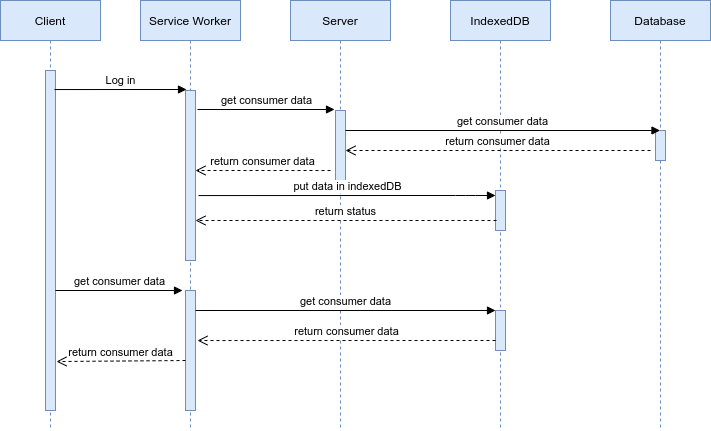
\includegraphics[width=0.9\textwidth]{images/flow}
						\caption{Diagramme de séquence du chargement des données}
						\label{fig:recuparation}
					\end{figure}
				
					Pour éviter d'avoir un dédoublement des données tout en conservant le principe de la base de données non-relationnelles, les données liées qui doivent s'afficher dans la même table sont toutes regroupées dans la même collection. Cela permet de conserver une grande vitesse de lecture des données et de ne pas ralentir le fonctionnement de l'application.
							
					Pour accélérer le processus, toutes les requêtes pour récupérer les données sont envoyées simultanément. Dès qu'une réponse est reçue, le service worker commence à ajouter les données dans l'indexedDB à l'aide de la bibliohtèque "Dexie.js" \cite{ref:dexie}. Pour ce faire, le service worker parcourt simplement tout le fichier \gls{json} reçu de l'\gls{api} et ajoute toutes les données présentes dans la collection adéquate.
				
				\subsubsection*{Envoi des données}
					Pour gérer l'envoi des données, la première solution envisagée a été d'utiliser la nouvelle \gls{api} "background-sync". Quand le service worker détecte qu'une requête réseau a échoué, il peut l'enregistrer comme un événement "sync" qui sera délivré quand le navigateur a récupéré la connexion. 
					
					L'avantage de cette solution est que le service worker peut envoyer les données même si la page a été fermée, ce qui permet d'éviter que les données restent indéfiniment non envoyées. Malheureusement, cette API n'est pour l'instant prise en charge que par certains navigateurs sur PC et Android mais n'est pas du tout prise en charge par iOS. Il a donc été décidé de laisser cette solution de côté.
					
					Du coup pour pallier ce problème, j'ai implémenté une solution qui est compatible avec tous les navigateurs. Lorsque l'utilisateur essaie d'ajouter, modifier ou supprimer des données, celles-ci sont dans un premier temps stockées dans l'indexedDB avant d'être envoyées. En cas de perte de connexion au serveur, cela permet de ne pas perdre les données que l'utilisateur vient d'encoder. Les données enregistrées dans l'indexedDB, le service worker va automiquement essayer de les envoyer. En cas de réussite, les données sont supprimées de l'indexedDB et en cas d'échec, les données restent stockées afin de pouvoir être envoyées plus tard. A chaque fois que l'utilisateur tentera de récupérer des données  sur le serveur, le service worker va d'abord essayer d'envoyer toutes les données en attente avant de récupérer les données du serveur. Cela permet d'éviter d'avoir des données non envoyées qui restent en attente.
					
					Si l'envoi des données réussit, le serveur répond avec les nouvelles données mises à jour. Lorsque le service worker reçoit cette réponse, il va mettre à jour les données qui sont dans le navigateur afin que l'utilisateur puisse voir directement les changements qui ont été éffectués même s'il utilise le mode hors-ligne de l'application \ref{fig:flows2}. La gestion des incohérences sera décrite plus loin dans la section \ref{sec:api}.
					
					\begin{figure}[H]
						\centering
						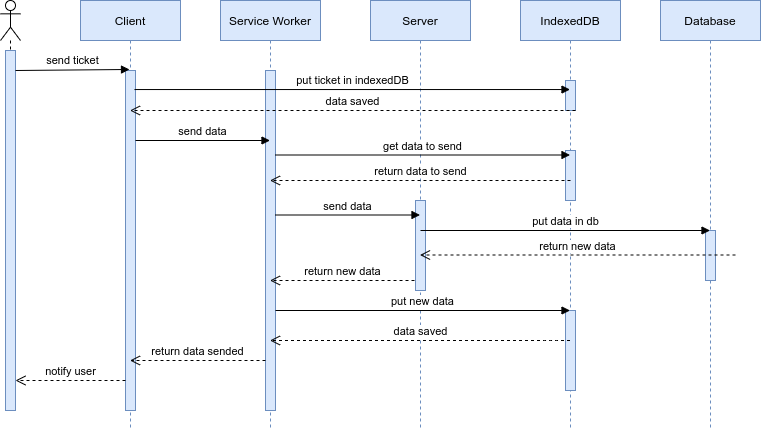
\includegraphics[width=0.9\textwidth]{images/flow2}
						\caption{Diagramme de séquence de l'envoi de données}
						\label{fig:flows2}
					\end{figure}
			
			\subsection*{Gestion des changements d'utilisateurs}		
				Afin de conserver une sécurité maximale, à chaque déconnexion d'un utilisateur, toutes les données et les fichiers (hors fichiers statiques) sont supprimés du navigateur. Il aurait été possible de ne pas supprimer ces données et de gérer des fonctionnalités multi-utilisateurs mais cela aurait impliqué de demander à l'utilisateur d'effectuer des démarches supplémentaires pour supprimer ces données. 
			
				De plus, à l'heure actuelle, chaque utilisateur possède son propre appareil; il n'est donc pas nécessaire de gérer le multi-utilisateur au détriment de la sécurité. En effet, en laissant les données dans le navigateur après la déconnexion d'un utilisateur, les données restent accessible via l'inspection du navigateur. Si une personne mal intentionnée utilisait l'appareil après un utilisateur, elle pourrait récupérer toutes les données stockées. 
				
			\subsection*{Sytème de notifications}
				Le système de notification, comme indiqué dans le tableau \ref{fig:moscow}, ne faisait pas partie des fonctionnalités à implémenter pour l'instant. Toutefois, un système local de notifications a tout de même été mis en place pour notifier l'utilisateur. Ces notification concernent:
				
				\begin{itemize}[noitemsep]
					\item La mise en attente d'envoi,
					\item La réussite ou l'échec d'envoi,
					\item La réussite ou échec de synchronisation,
					\item Autres informations.
				\end{itemize}								
				
		
		\section{Interface utilisateur}
			L'interface utilisateur existante a dû subir quelques modifications afin d'accueillir le mode hors-ligne. La nouvelle application permet en effet deux modes différents d'utilisations.
			
			\subsection*{Changement de mode}
				Afin de passer d'un mode d'utilisation à l'autre, un bouton switch a été ajouté en haut de l'interface, à coté de la cloche de notification. Quand ce bouton affiche un rond vert, cela signifie que l'application est en mode en ligne. Lorsque le rond est noir, cela signifie que l'application est en mode hors-ligne.
				
				 A coté de ce bouton switch a été ajouté un autre bouton permettant de mettre à jour toutes les données présentes dans le navigateur, cela afin de ne pas obliger l'utilisateur à mettre à jour toutes les tables une par une. A droite de ce bouton, se trouvent la date et l'heure des données les plus anciennes présentes dans le navigateur. Lorsque l'utilisateur se connecte à l'application, la phrase "pas encore de données" s'affiche, aucune donnée n'étant encore chargée. Cela permet à l'utilisateur de savoir à quel point les données du navigateur sont à jour.
				
				\begin{figure}[H]
					\centering
					
\includegraphics[width=0.5\textwidth]{images/buttons}
					\caption{Nouveaux boutons}
					\label{fig:buttons}
				\end{figure}
			
			\subsubsection*{Mode en ligne}
				Il s'agit du mode par défaut lorsque l'utilisateur se connecte à l'application. Il faut du temps pour que toutes les données soient chargées dans le navigateur afin que l'application puisse fonctionner en mode hors-ligne. Programmer ce mode par défaut permet donc à l'utilisateur d'utiliser l'application bien que toutes les données ne soient pas encore chargées. Dans ce mode, les différentes pages vont récupérer les données à afficher directement dans la base de données grâce à l'\gls{api} et pas dans l'indexedDB du navigateur. 
				
				Ce mode est très utile s'il est nécessaire d'avoir accès aux dernières données disponibles et quand la connexion le permet. Pour de plus amples informations sur ce mode de fonctionnement vous pouvez consulter le mémoire de la première version de l'application \cite{ref:haitiwater}.
			
			
			\subsubsection*{Mode hors-ligne}
				Ce mode permet d'afficher les données qui sont présentes localement dans l'indexedDB du navigateur. C'est dans ce mode que l'utilisateur pourra utiliser l'application lorsque la connexion au serveur n'est pas disponible. En passant en mode hors-ligne, la couleur du bandeau de l'application passe du bleu au rouge, signifiant que l'utilisateur est bien dans le mode hors-ligne (cf. figure \ref{fig:mode}). Les données ne sont donc plus récupérées sur le serveur.
								
				\begin{figure}[H]
					\centering
					\begin{subfigure}[b]{0.3\textwidth}
  						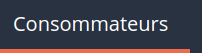
\includegraphics[width=1\linewidth]{images/consumer_blue}
  						\caption{Online}
					\end{subfigure}%
					\begin{subfigure}[b]{0.332\textwidth}
  						
\includegraphics[width=1\linewidth]{images/consumer_red}
  						\caption{Offline}
					\end{subfigure}
					\caption{Modes d'utilisation}
					\label{fig:mode}
				\end{figure}
			
				Dans ce mode, lorsque des requêtes n'ont pu être envoyées, les données concernées apparaitront en mauve dans le tableau pour que l'utilisateur sache que des modifications sont en attente. Quand les données ont été envoyées et que le serveur a répondu, les données hors-ligne modifiées sont mises à jour localement pour refléter les changements effectuer sur le serveur. Elles n'apparaissent plus en mauve dans les tables (cf. figure \ref{fig:purple}). 
				
				\begin{figure}[H]
					\centering
					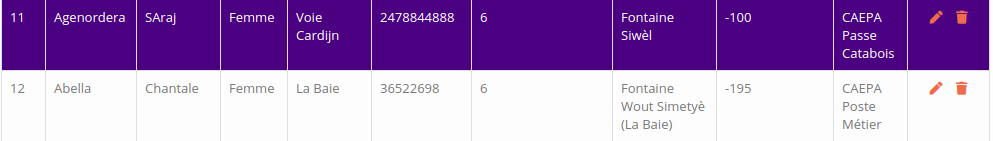
\includegraphics[width=1\textwidth]{images/purple}
					\caption{Données en attente de synchronisation}
					\label{fig:purple}
				\end{figure}
				
							
			\subsection*{Module à synchroniser}
				Il s'agit d'un nouveau module qui a été ajouté pour les besoins du mode hors-ligne. Dans ce module, l'utilisateur retrouve un tableau qui reprend toutes les données qui n'ont pas été envoyées vers le serveur. Dans ce tableau, il peut retrouver différentes informations (cf. figure \ref{fig:tosync}).
				
				\begin{figure}[H]
					\centering
					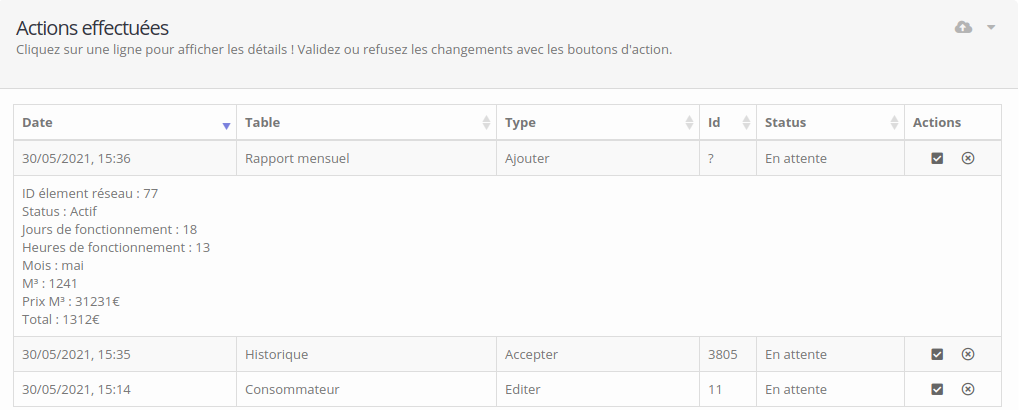
\includegraphics[width=1\textwidth]{images/tosync}
					\caption{Module "A synchroniser"}
					\label{fig:tosync}
				\end{figure}
							
				L'utilisateur peut choisir de supprimer des données du tableau, auquel cas il ne pourra plus essayer de les envoyer, celles-ci étant supprimées de l'indexedDB. Une alternative consiste à envoyer une donnée en particulier ou toutes en même temps grâce au bouton situé dans l'en-tête du tableau.
			
		
		\section{Serveur}
		\label{sec:serveur}
			Dans cette partie, je vais décrire le fonctionnement du serveur. Je ferai d'abord un résumé sur son fonctionnement de base et j'expliquerai ensuite les changements apportés afin de récupérer les données nécessaires à l'affichage hors-ligne.
			
			\subsection*{Requêtes}
				Une requête est une demande que le navigateur envoi au serveur afin de récupérer différents types de fichiers ou de données. Le serveur permet de gérer trois types de requêtes différentes.
				
				\begin{description}
					\item[Fichiers statiques] Le serveur répond a ces requêtes en envoyant tous les fichiers de style et Javascript.
					\item[Documents] Le serveur renvoie à l'utilisateur les pages l'HTML à afficher. Ce sont les documents qui vont importer les fichiers statiques.
					\item[Données] Le serveur renvoie toutes les données demandées. Pour ce faire l'\Gls{orm} est utilisé. Django se charge d'effectuer la connexion avec la base de données et de lui renvoyer toutes les requêtes. Cela permet d'interagir avec les données sans avoir à toucher au SQL.
				\end{description}

				Les fichiers statiques et les documents permettent au navigateur d'afficher toute l'interface graphique. Chaque module du serveur permet de desservir une page de l'application. Ces pages peuvent avoir des éléments personnalisés en fonction de l'utilisateur connecté. Les données sont téléchargées après le chargement de la page.
				
				N'étant pas l'objet de mon mémoire, le fonctionnement global du serveur n'a pas été modifié.
				
				
			\subsection*{API}
				\label{sec:api}
				Le module \gls{api} a subi quelques modifications afin que le service worker puisse télécharger toutes les données dont il a besoin lorsque la connexion au serveur n'est pas disponible. La version de base du serveur ne permettait que le téléchargement d'une partie des données, celle à afficher directement par la page. Par exemple, lorsque l'application doit afficher la page "Consommateurs", l'\gls{api} ne répond que les dix éléments devant être affichés sur la page et une nouvelle requête est nécessaire à chaque fois que des données différentes sont souhaitées (la page 2 du tableau par exemple).
				
				Pour résoudre ce problème, j'ai implémenté des fonctions supplémentaires qui permettent de récupérer en une seule requête toutes les données nécessaires à l'affichage d'une table. Cela permet au service worker de récupérer toutes les données dont il a besoin afin de les mettre dans l'indexedDB lors de son installation. Ces nouvelles fonctionnalités nécessitent toujours que l'utilisateur soit connecté.
				
				De plus, afin d'aider le mode hors-ligne à être plus précis dans l'affichage des données, lorsqu'une requête d'ajout, de modification ou de suppression de données est envoyée au serveur, ce dernier ne vas pas répondre qu'avec un status 200 (signifiant que les changements ont bien été pris en compte), mais va également renvoyer la donnée modifiée au format \gls{json} afin que le service worker puisse mettre à jour directement les données localement.
				
				Une autre difficulté se manifeste quand les utilisateurs ne sont plus connectés au serveur; il est possible qu'ils modifient la même donnée sans concertation.
				
				Pour l'instant le travail des gestionnaires de fontaines doit être validé par un gestionnaire de zone via le module "Historique" décrit au point \ref{sec:historique}. Le serveur accepte les données comme elles viennent et les ajoute dans la liste des données en attente de traitement. Si des incohérences apparaisent, le gestionnaire responsable contacte les gestionnaires concernés par l'incohérence et la corrige en approuvant ou en rejetant les modifications apportées. Pour l'instant, la donnée qui apparait sur le serveur est celle de l'utilisateur qui a envoyé ces données en dernier.
			
			
			
			
			
%---------------------------------------------------------------------------------------------------------
	\chapter{Validation}
		La validation a pour objectif de tester le bon fonctionnement et la qualité du produit "fini". Pour effecuter cette validation, deux types de test ont été utilisés: d'une part, des tests automatisés afin de pouvoir tester le fonctionnement des différentes fonctions implémentées et, d'autre part, des tests  de validation avec des utilisateurs réels afin de tester le fonctionnement global de l'application ainsi que son intuitivité.

		

		\section{Vérifications automatiques}
			Pour tester l'application de façon automatique, j'ai utilisé des tests unitaires. Ces tests ont pour objectif de vérifier le bon fonctionnement d'une partie précise d'une application (unité ou module). Ils assurent qu'une méthode qui peut être utilisée par un utilisateur fonctionne de la manière prévue. Dans le cas présent, toutes les interactions entre l'application et l'utilisateur se font à l'aide soit de requêtes envoyées directement au serveur, soit de requêtes faites au service worker. J'ai donc décidé de compléter les tests unitaires qui étaient déjà présents pour la partie serveur et de créer une batterie de tests unitaires pour le service worker.

			Pour de plus amples informations le mémoire en lien avec la création de l'application est en consultation libre \cite{ref:haitiwater}. Les tests que j'ai ajoutés au niveau des reqûetes au serveur couvrent les méthodes de récupération des données utilisées par le service worker. Je vérifie que les données récupérées sont uniquement celles auxquelles l'utilisateur a accès et que celles-ci sont complètes.
			
			En ce qui concerne les tests sur le service worker, ceux-ci couvrent toutes les fonctions de récupération et d'envoi de données de et vers la base de données ainsi que la gestion de toute page mise en cache pour leur affichage en mode hors-ligne.

		\section{Vérifications utilisateurs réels}
.			Lors de cette phase, l'application a été présentée a des utilisateurs (certains ayant utilisés la première version, d'autres non) afin qu'ils puissent fournir le feedback nécessaire à son évolution. Trois apsects ont été testés: la compréhension des différents modes, la gestion des données en cas de perte de connexion au serveur et les modifications de l'interface. Le but est d'identifier les problèmes présents dans l'application et de réfléchir à leur solution. Dans cette optique, avoir des avis externes sur l'application permet de l'améliorer drastiquement.
			
			Les tests se sont déroulés en présentiel avec les participants ou via Microsoft Teams en fonction de la disponibilité des personnes et des mesures sanitaires en vigueur. Un groupe de dix personnes venant d'horizons différents et ayant des compétences diverses et variées ont testé l'application.


			\subsection*{Méthodologie}
				\label{sec:methodo}
				La méthodologie qui a été utilisée pour faire passer ces tests est restée la même que pour le mémoire précédent \cite{ref:haitiwater}. Celle-ci a été adaptée aux nouvelles fonctionnalités développées lors de ce mémoire afin que ce test reste cohérent avec le travail réalisé. Le fait d'utiliser le même type de test permet de voir concrètement comment évolue le niveau de satisfaction des utilisateurs après cette deuxième année de développement.
				
				Les séances de validation se sont déroulées en partie physiquement et en partie à distance via le logiciel Microsoft Teams, ces logiciels permettant de faire de la transmission vocale et du partage d'écran. L'étudiante de Haïti m'a également aidé à faire passer les tests aux différents utilisateurs présents là-bas, cela afin de me faciliter la tâche à cause du décalage horaire.
				
				Les testeurs ont d'abord reçu une brève introduction à l'application et sur le but de la séance de validation. Je leur ai ensuite remis un à trois scénarios à réaliser durant la séance. Ces scénarios contiennent une brève introduction au contexte et une liste de tâches à compléter. Après la lecture du scénario, je répondais aux questions éventuelles. Ensuite, l'utilisateur est laissé seul pour faire sa tâche. S'il avait des questions pendant le déroulement de la tâche, je lui donnais une indication pour l'aider.
				
				Après la réalistion de ses tâches, le testeur a reçu une série de 21 questions. Ces questions sont regroupées par thème.
				\begin{description}
					\item[Tâches] Ces questions permettent de savoir si les tâches à accomplir étaient suffisament claires.
					\item[Fonctionnalités]  Ces questions permettent de savoir si l'interface de l'application permet une utilisation simple des fonctions implémentées.
					\item[Usabilité] Ces questions permettent d'avoir le ressenti de l'utilisateur et de récolter des indices quant à une possible amélioration de l'application au niveau l'usabilité.
					\item[Esthétique] Ces questions permettent de savoir si le design de l'application plaît aux utilisateurs.
				\end{description}

				Pour répondre aux différentes questions, j'ai utilisé l'échelle de Likert. L'échelle de Likert est une échelle de mesure qui comprend dans ce cas cinq degrés de réponse. Elle est souvent utilisée dans les questionnaires. Elle permet de jauger le niveau d'accord ou de désacord d'une affirmation \cite{ref:likert}.
				
	
			\subsection*{Résultats obtenus}
				Le graphe \ref{fig:validation} reprend les résultats des 21 questions posées aux utilisateurs pour évaluer leur niveau de statisfaction sur les thèmes cité à la section \ref{sec:methodo}. Les résultats sont dans l'ensemble très positif. Cela montre que les utilisateurs apprécient cette nouvelle version de l'application et la trouve simple à utiliser. 
			
				\begin{figure}[H]
					\centering
					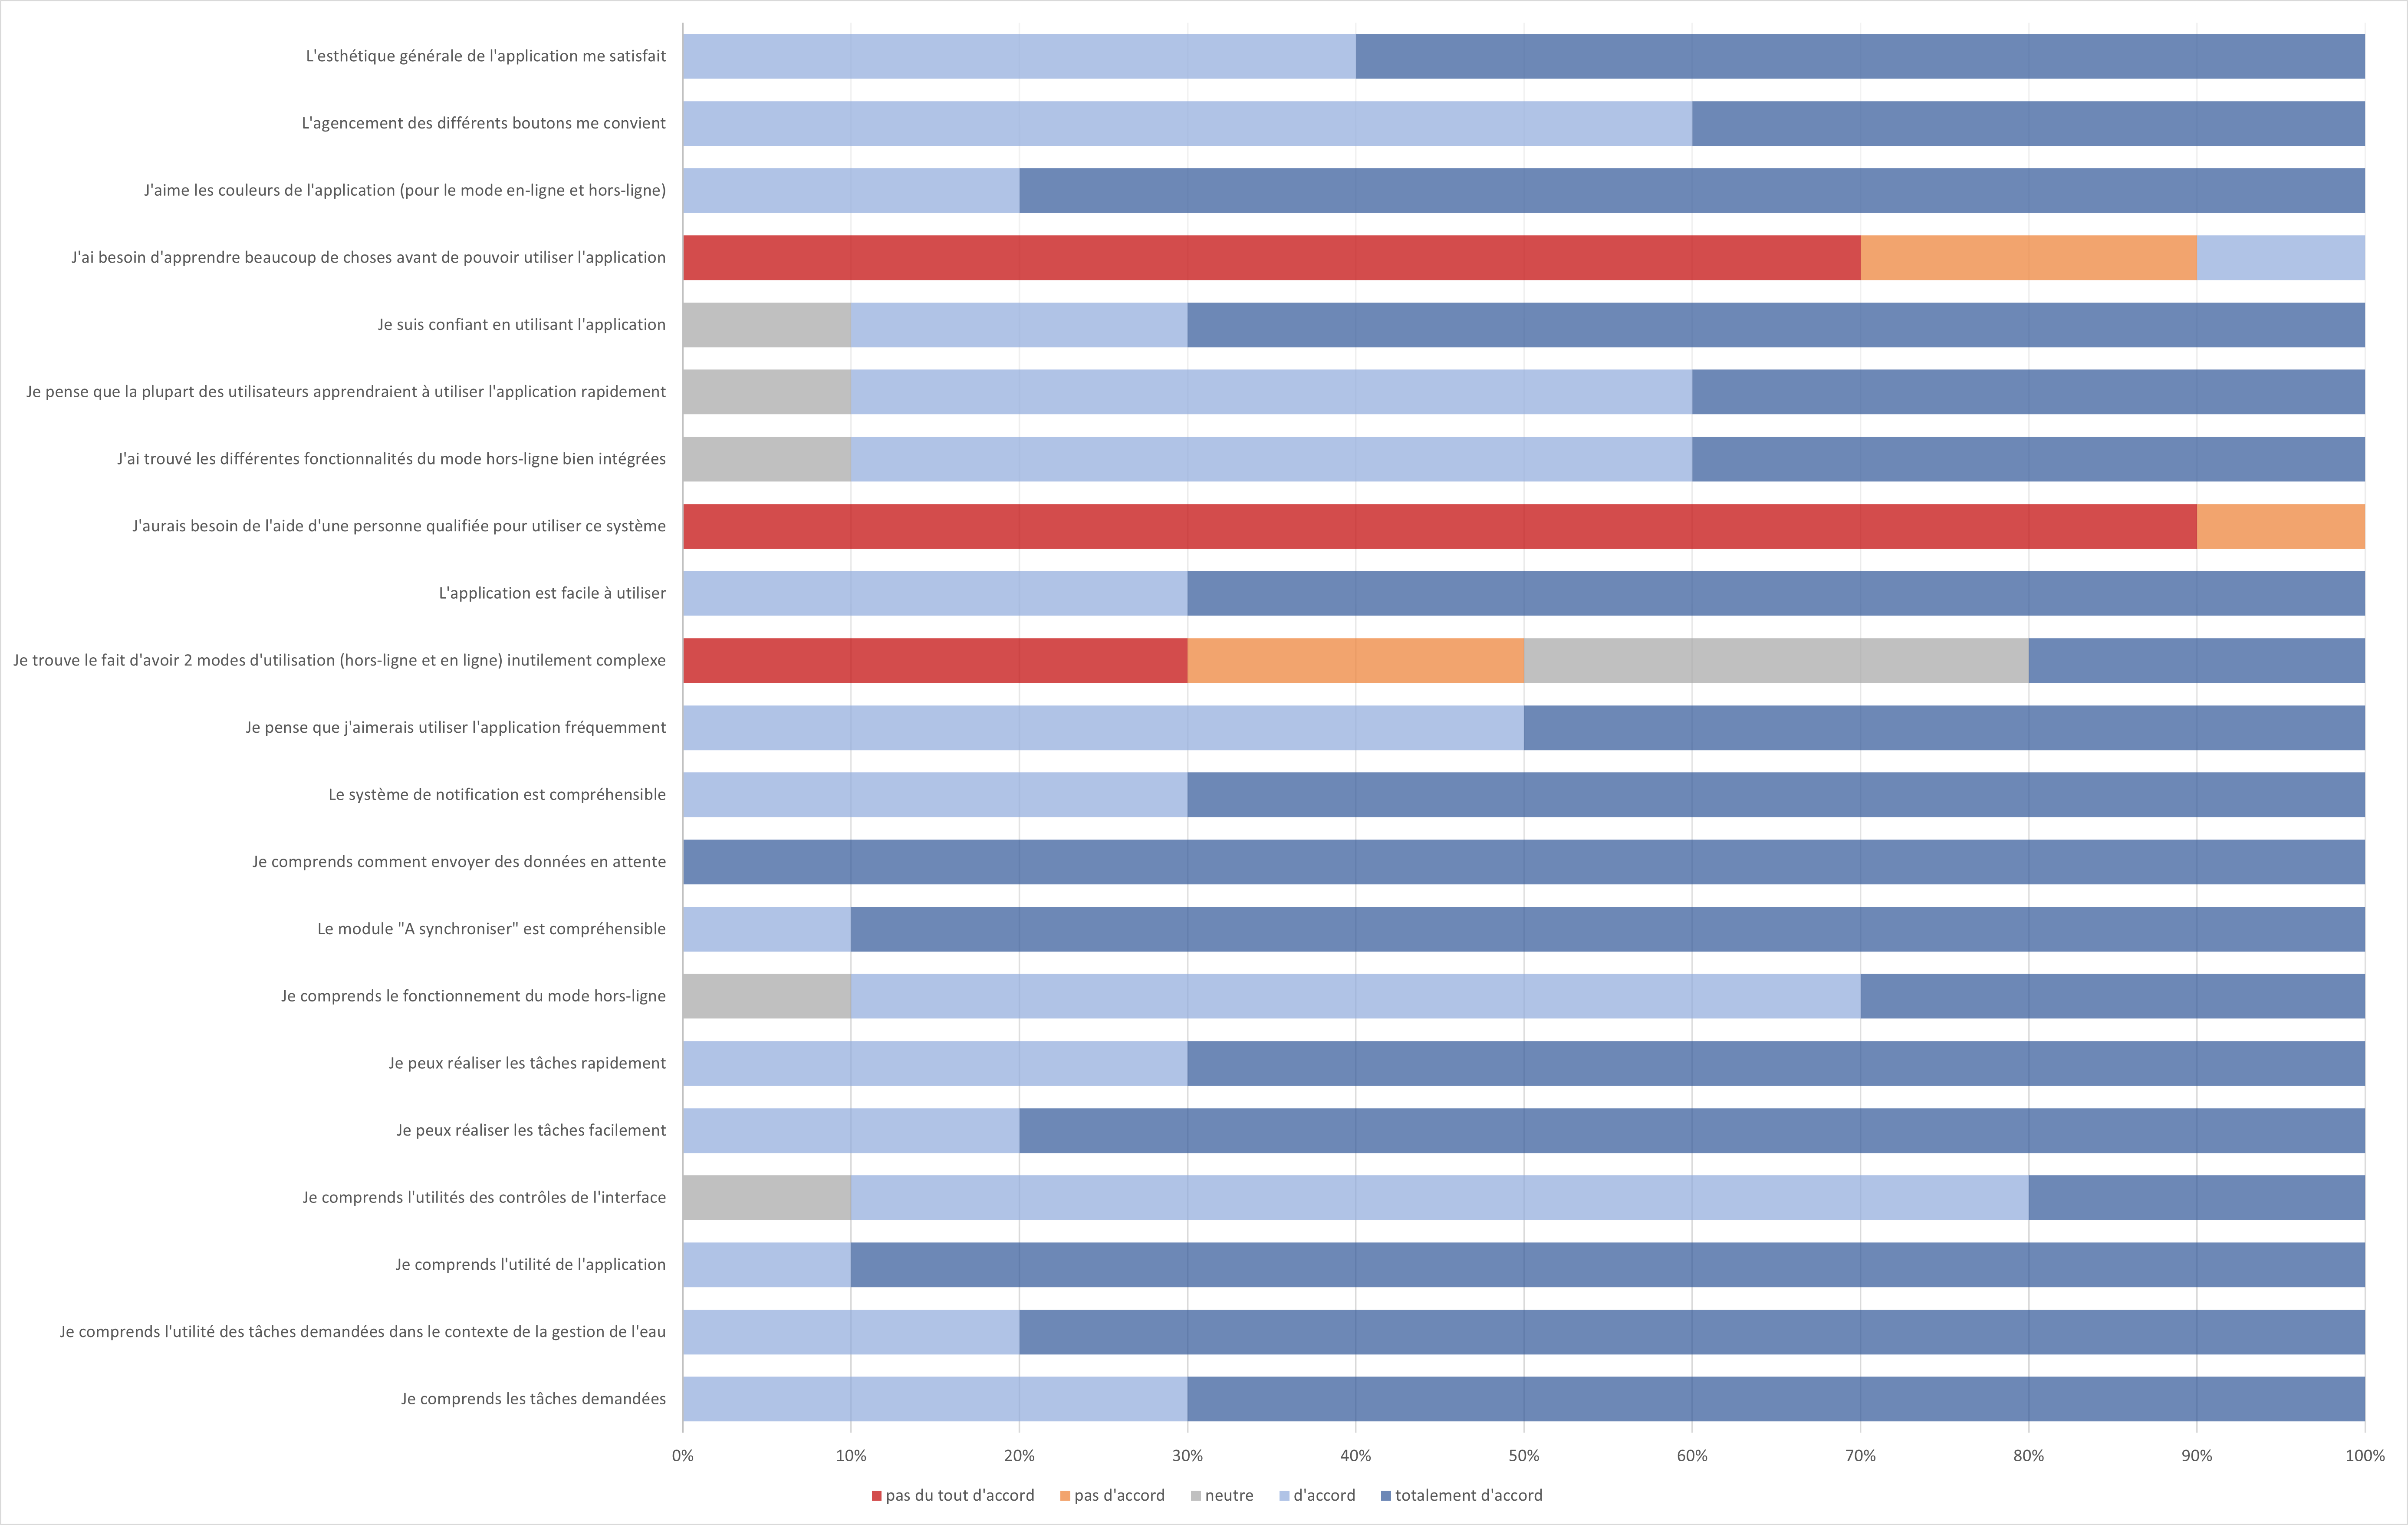
\includegraphics[width=1\textwidth]{images/validation}
					\caption{Données de validation concernant le test de l'application}
					\label{fig:validation}
				\end{figure}
		
				Il y a cependant un point qui n'a pas mis tout le monde d'accord; à l'affirmation "Je trouve le fait d'avoir deux modes d'utilisation inutilement complexe", le panel de réponse est hétérogène. Cette solution ne fait pas l'unanimité et une évolution de la gestion des modes reste donc nécessaire.
		
			\subsection*{Modifications apportées}
				Grâce aux différents commentaires reçu des utilisateurs, certains changements mineurs ont été effectués. Le premier est l'ajout d'un mode d'emploi sur la page d'accueil pour expliquer le fonctionnement du mode hors-ligne.
				Le second est l'ajout de notification lorsque les données sont en cours d'envoi. 
				Les autres modifications qui peuvent être apportées seront décrites dans la section \ref{sec:proposition}.
				
				

%------------------------------------------------------------------------------------------------------
	\chapter{Améliorations futures}
		Malgré les deux années de travail effectuées par les trois anciens mémorants \cite{ref:haitiwater} et moi-même, le projet est loin d'être terminé. Même si l'application peut commencer à être deployée dès maintenant, comme tout projet de développement de grande ampleur, HaïtiWater devra être suivie afin d'être mise à jour et maintenue pour un bon fonctionnement au quotidien. 

		\section{Suite du projet}
			\label{ref:suite_projet}
			S'atteler à la finition de l'application HaïtiWater sera la priorité des futures équipes de développement. En l'état actuel, l'application peut déjà servir aux acteurs locaux afin de travailler sur le terrain. Cependant, la base de l'application peut toujours être optimisée pour être encore plus sûre et réactive.		
			Comme évoqué par mes prédécesseurs \cite{ref:haitiwater}, une des tâches importantes pour le futur reste l'automatisation des rapports en agrégeant les données et en développant une meilleure visualisation de celles-ci. Une autre amélioration évoquée par mes prédécesseurs est le développement d'un serveur mail et d'un serveur SMS dédié de sorte que le serveur de l'application ne soit pas surchargé lors de l'envoi de ceux-ci.
			
			L'application HaïtiWater est en cours de déploiement sur un serveur haïtien et devrait être disponible dans les semaines à venir. Cette migration devrait améliorer le temps de chargement de l'application pour les acteurs locaux. Le serveur qu'ils utiliseront devrait d'ailleurs être plus performant que celui utilisé en Belgique. Pour l'instant, il s'agit d'un serveur dual-core de 2 GHz avec 2 Go de mémoire vive. Les temps de chargement devraient donc être drastiquement réduits graĉe à un serveur plus puissant. 
			
			Une dernière amélioration serait l'optimisation de l'\gls{api} afin que la récupération des consommateurs soient plus rapide.
		
			Actuellement l'application prend du temps à être complétement chargée pour une utilisation hors-ligne. Ce délai empêche l'utilisation du mode hors-ligne avec Mozilla Firefox pour les utilisateurs ayant beaucoup de consommateurs, le problème étant que ce navigateur stoppe le service worker bien avant d'avoir reçu la réponse du serveur.
					

		\section{Défis rencontrés}
			La difficulté la plus importante lors de ce projet a été la méconnaissance de la technologie utilisée et le fait qu'il y a encore peu d'aide sur internet. De plus, les service workers sont encore en cours de développement; l'ensemble de leurs fonctionnalités ne sont pas supportées par tous les navigateurs. Il a donc fallu trouver des solutions pour que l'application puisse rester fonctionnelle même si l'utilisateur emploie un navigateur qui ne prend pas en charge les service workers. 
			
			Une dexième difficulté était mon manque d'expérience. En effet, je ne m'étais jamais engagé dans un projet d'une telle envergure. Une période conséquente d'apprentissage autonome avant de se lancer dans le projet a été nécessaire. Heureusement, les anciens mémorants étaient assez disponibles et m'ont aidé à résoudre les problèmes rencontrés.
			
			Le dernière difficulté rencontrée a été une motivation en dents de scie. Comme tout le mode, mes conditions de vie (isolement sociel) et de travail (manque d'objectifs à court terme) ont été bousculées par les mesures sanitaires faisant suite à la pandémie du COVID-19. 
			

		\section{Propositions}
		\label{sec:proposition}
			L'application HaïtiWater peut encore évoluer de nombreuse manières. Une demande a été faite pour intégrer un module \Gls{citizen} afin que les consommateurs du réseau de distribution d'eau potable puissent signaler eux-mêmes les différents problèmes présents sur ce réseau ainsi que consulter leurs factures et consommations.
			
			En l'état l'application a été optimisée grâce à la mise en cache de tous les fichiers nécessaires à l'affichage des pages et à la copie locale de la base de données. Cependant, une amélioration possible serait l'utilisation d'un \gls{framework} frontend (Vue, React ou Angular) afin d'améliorer la réactivité globale de l'interface, ces \gls{framework} s'intégrant parfaitement aux \gls{pwa}.
			
			La gestion des données stockées localement pourrait être améliorée afin de ne plus proposer deux modes différents de fonctionnement de l'application mais un seul mode dans lequel toutes les données seraient synchronisées automatiquement au fur et à mesure que l'utilisateur adresse ses requêtes au serveur.
			
			Une autre évolution possible serait d'ajouter un système de notifications basé sur le serveur plutôt que localement. Pour l'instant, ce système de notifications n'est pas du tout synchronisé avec le serveur et ne sert qu'à l'affichage de certaines informations stockées dans le navigateur. Un service de messagerie interne à l'application pourrait également aider les utilisateurs à communiquer entre eux. Ce système de notifications mis en place, la gestion des incohérences de données décrite dans la section \ref{sec:api} pourra être améliorée afin d'envoyer directement des avertissements aux deux utilisateurs qui ont modifié les mêmes données hors-ligne.
		
			Enfin, les modules existants pourraient être améliorés afin de proposer différentes façons d'interagir avec les données. Par exemple, il serait intéressant de pouvoir exporter la base de données sous forme de fichier excel ou d'intégré d'avantages d'outils graphiques rendant les informations plus visuelles.




%-----------------------------------------------------------------------------------------------------
	\chapter{Conclusion}
		Grâce à la réalisation de mon mémoire, j'ai pu m'inscire dans un projet d'une grande envergure, mettre en pratique les compétences acquises au cours de mes études et aquérir une expérience non négligeable dans le développement d'une application web de grande ampleur.
		
		Lors de la phase de validation avec des utilisateurs réels, l'application HaïtiWater et son nouveau mode hors-ligne ont sucité un intéret certain chez les testeurs. Leurs retours étaient plûtot positifs. J'ai bon espoire que l'application finira par être utilisée par les acteurs locaux de manière régulière, voire quotidienne, et qu'elle continuera à évoluer.
		
		Avec plus de temps et une plus grande lattitude dans les tâches à accomplir, j'aurais pu mettre en place les améliorations précitées à la section \ref{sec:proposition}. De plus, je regrette de ne pas voir pu procéder à la validation plus tôt, ce qui m'a limité dans le champs des améliorations. Je n'ai malheureusement pu apporter que des améliorations mineures.

		Cette expérience d'apprentissage m'aura permis de mieux définir dans quel domaine de l'informatique je désire travailler après l'obtention de mon diplome. De plus, cela m'a permis de découvrir quelles technologies je souhaiterai investiguer et maîtriser dans un futur plus ou moins proche.
		
		

	\bibliographystyle{plain}
	\bibliography{bibliography.bib}
	
	
	\appendix
	
		\chapter{Diagramme de Gantt}
		
			\begin{figure}[H]
					\centering
					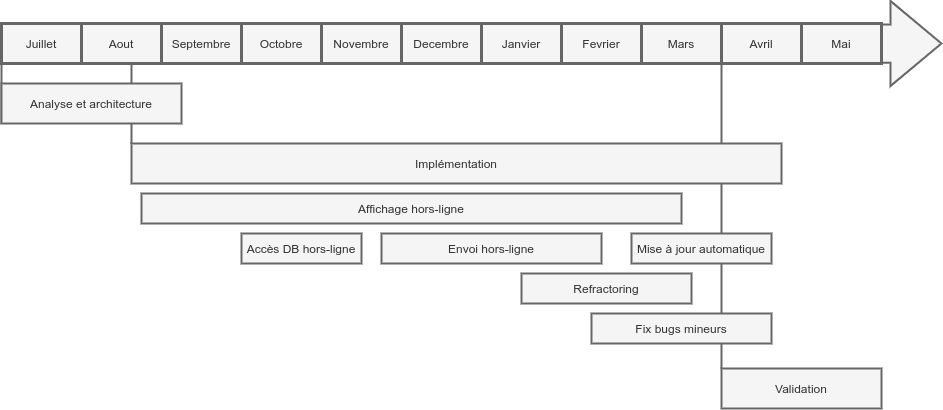
\includegraphics[width=1\textwidth]{images/Gantt}
					\caption{Diagramme de Gantt}
					\label{fig:Gantt}
			\end{figure}
				

				
			\paragraph*{Analyse et architecture}
			La première phase de mon mémoire est une phase d'analyse permettant la determination des technologies a utiliser selon les différentes fonction à implémenter. C'est dans cette phase qu'il y a eu beaucoup de discussions avec l'étudiante venue de Haïti.
		
			\paragraph*{Implémentation} 
			Le deuxième phase de mon mémoire, l'implémentation, est la plus conséquente; c'est ici que toutes les décisions prises durant la phase d'analyse se sont mises en place. Cette phase se divise en plusieurs phases qui représentent les différentes fonctionnalités produites durant le mémoire. 
			
			\paragraph*{Validation}
			La phase de validation n'intervient que tard dans le déroulement de mon mémoire. Pour cause, des facteurs tels que la méconnaissance de la technologie à utiliser et le temps de déploiement de la nouvelle version de l'application sur les serveurs haïtiens ont retardé sa mise en oeuvre.	
		
		\chapter{Documents de validation}
			\section*{Questionnaire}
				Voici les 21 questions posées aux utilisateurs pendant la validation. Elles sont triées par thème.
				\subsection*{Tâches}
					\begin{itemize}
						\item Je comprends les tâches demandées.
						\item Je comprends l'utilité des tâches demandées dans le contexte de la gestion de l'eau.
						\item Je comprends l'utilité de l'application.
					\end{itemize}
					
				\subsection*{Fonctionnalités}
					\begin{itemize}
						\item Je comprends l'utilités des contrôles de l'interface.
						\item Je peux réaliser les tâches facilement.
						\item Je peux réaliser les tâches rapidement.
						\item Je comprends le fonctionnement du mode hors-ligne.
						\item Le module "A synchroniser" est compréhensible.
						\item Je comprends comment envoyer des données en attente.
						\item Le système de notification est compréhensible.
					\end{itemize}
				\subsection*{Usabilité}
					\begin{itemize}
						\item Je pense que j'aimerais utiliser l'application fréquemment.
						\item Je trouve le fait d'avoir 2 modes d'utilisation (hors-ligne et en ligne) inutilement complexe.
						\item L'application est facile à utiliser.
						\item J'ai trouvé les différentes fonctionnalités du mode hors-ligne bien intégrées.
						\item Je pense que la plupart des utilisateurs apprendraient à utiliser l'application rapidement.
						\item Je suis confiant en utilisant l'application.
						\item J'ai besoin d'apprendre beaucoup de choses avant de pouvoir utiliser l'application.
						\item J'ai besoin de l'aide d'une personnée qualifiée pour utiliser ce système.
					\end{itemize}
				\subsection*{Esthétique}
					\begin{itemize}
						\item J'aime les couleurs de l'application (pour le mode en-ligne et hors-ligne).
						\item L'agencement des différents boutons me convient.
						\item L'esthétique générale de l'application me satisfait.				
					\end{itemize}
					
\newpage
			\section*{Scenario 1 - Gestion hors-ligne}
				\begin{description}
					\item[Rôle] Administrateur principale
					\item[Objectif] Créer un nouveau gestionnaire et lui assigner une zone. 
					\item[Prérequis] La zone de l'artibonite dans la DB.
					\item[Contexte] Vous êtes Claude, membre de l’ONG Protos. L’application HaïtiWater est déjà utilisée dans plusieurs départements d’Haïti et le département de l’Artibonite, zone nouvellement créée, vous souhaitez créer un nouveau gestionnaire de zone et l’assigner à celle-ci. En tant que responsable de l’application, vous devez permettre au responsable de la gestion de l’eau en Artibonite de se connecter à l’application et de gérer son réseau. Vous devez donc créer un nouveau gestionnaire et lui assigner la zone d’Artibonite. Lorsque vous voulez encoder les informations, le réseau disparait soudainement. 
				\end{description}
							
				\subsubsection*{Informations nécessaires}
					\begin{itemize}[noitemsep, label={}]
						\item \textbf{Utilisateur} ***********
						\item \textbf{Mot de passe} ***********
					\end{itemize}

					
				\subsubsection*{Tâche 1}
					\begin{itemize}
						\item Connectez-vous à l’application avec votre compte de gestionnaire : Protos.
						\item Pendant que les données charges (indiqué en haut de l’écran), voyagez dans l’application.
						\item Vous êtes dans la zone de l’Artibonite pour rencontrer le nouveau gestionnaire et l’encoder.
						\item Vous allez dans la partie gestion et là la connexion au serveur disparait.
						\item Passez l’application en mode hors-ligne.
						\item Encodez le nouveau gestionnaire et assignez-lui sa zone (vous pouvez entrer vos propres données ou des données fictives).
						\item Vérifiez dans la partie "A synchroniser" que les données ont bien été enregistrées pour être envoyées ultérieurement.
					\end{itemize}
					
				\subsubsection*{Tâche 2}
					\begin{itemize}
						\item Le réseau est revenu.
						\item Allez dans la partie à synchroniser.
						\item Vérifiez que les données encodées précédemment sont correctes. 
						\item Envoyez les données vers le serveur. 
						\item Retournez dans la partie dans la partie gestion et vérifier que vos changements ont bien été pris en compte. 
					\end{itemize}
			

\newpage
			\section*{Scenario 2 - Utiliser les tables hors-ligne}
				\begin{description}
					\item[Rôle] Gestionnaire de zone
					\item[Objectif] Imprimer la liste des tous les éléments (fontaines, kiosques, ...) du réseau de la zone CAEPA Passe Catabois classés par volume de sortie total.
					\item[Prérequis] Plusieurs zones avec plus de dix fontaines par zone. 
					\item[Contexte] Vous êtes Dominique, gestionnaire de zone et supervisez les opérations au niveau national. Cette semaine, une réunion a lieu pour décider des budgets alloués à la maintenance des fontaines de la zone de l’Ouest. Pour vous aider à allouer les fonds de manière équitable, vous avez besoin de la liste des installations de cette zone, classées par nombre d’utilisateurs décroissant. Malheureusement le réseau vous a abandonné. 
				\end{description}
							
				\subsubsection*{Informations nécessaires}
					\begin{itemize}[noitemsep, label={}]
						\item \textbf{Utilisateur} ***********
						\item \textbf{Mot de passe} ***********
					\end{itemize}
					
				\subsubsection*{Tâche 1}
					\begin{itemize}
						\item Connectez-vous à l’application avec votre compte de gestionnaire. 
						\item Pendant que les données charges (indiqué en haut de l’écran), voyagez dans l’application. 
						\item Vous voulez aller récupérer les données mais le réseau internet n’est plus accessible. 
						\item Passez en mode hors-ligne. 
						\item Rendez-vous dans votre page de gestion et trouvez un moyen de filtrer les éléments pour ne conserver que ceux de la zone CAEPA Passe Catabois. 
						\item Triez les éléments par nombre d’utilisateurs décroissant. 
						\item Imprimez les éléments en vous assurant d’avoir la liste complète affichée. Vous pouvez vous arrêter une fois que le navigateur vous propose d’imprimer le bon document, il n’est pas nécessaire de l’imprimer physiquement. 
					\end{itemize}
					
				\subsubsection*{Tâche 2}
					\begin{itemize}
						\item Le réseau est de retour. 
						\item Vous désirez mettre à jour la table des éléments réseau tant que vous avez accès à internet. 
						\item llez dans la section éléments du réseau et synchronisez la table. 
						\item Attendez que la table soit synchronisée. 
					\end{itemize}
			
			
\newpage
			\section*{Scenario 3 - Ajouter des paiements hors-ligne}
				\begin{description}
					\item[Rôle] Gestionnaire de fontaine 
					\item[Objectif] Ajouter des paiements pour deux consommateurs lorsque vous n’avez pas de connexion. 
					\item[Prérequis] Deux consommateurs dans la zone utilisateur (noms ci-dessous).  
					\item[Contexte] Vous êtes John, un membre de l’administration du système HaïtiWater. En visite dans un village, vous en profitez pour aider un gestionnaire de fontaine local dans son encodage des paiements. Deux consommateurs viennent vous voir, billets en main, et viennent payer leur redevance. Le réseau étant assez instable dans la région, vous utilisez le mode hors-ligne pour encoder les paiements. Une fois le réseau revenu vous envoyez alors les données encodées vers le serveur. 
				\end{description}
							
				\subsubsection*{Informations nécessaires}
					\begin{itemize}[noitemsep, label={}]
						\item \textbf{Utilisateur} ***********
						\item \textbf{Mot de passe} ***********
					\end{itemize}
					
				\subsubsection*{Tâche 1}
					\begin{itemize}
						\item Connectez-vous à l’application. 
						\item Pendant que les données charges (indiqué en haut de l’écran), voyagez dans l’application. 
						\item Allez dans la partie financière de l’application. 
						\item Soudainement vous n’avez plus d’accès au réseau et vous passez donc en mode hors-ligne. 
						\item Monsieur Stevene  Ivener vous donne 150 (gourdes), entrez ce paiement dans l’application. 
						\item A sa demande, informez MadNotification Consommateurs ame Honoré Roselie de l’état général de ses paiements (dites à votre examinateur à combien de Gourdes s’élève son retard ou son avance sur les paiements). 
						\item Madame Honoré Roselie vous donne 100 (gourdes), encodez son paiement. 
					\end{itemize}
					
				\subsubsection*{Tâche 2}
					\begin{itemize}
						\item Allez vérifier dans la partie “à synchroniser” que vous données ont bien été encodées. 
						\item Envoyez les données en attente. 
						\item Retournez dans la partie paiement. 
						\item Vérifiez que les paiements ont bien été ajoutés. 
					\end{itemize}
			
			
\newpage
			\section*{Scenario 4 - Gestionnaire de fontaines hors-ligne}
				\begin{description}
					\item[Rôle] Gestionnaire de fontaine 
					\item[Objectif] Ajouter des consommateurs et encoder un rapport mensuel lorsque le réseau est instable. 
					\item[Prérequis] Un gestionnaire de fontaines et ses éléments du réseau : une fontaine, un kiosque et une prise individuelle. 
					\item[Contexte] Vous êtes Frédérique, gestionnaire de fontaine. Vous avez la responsabilité de trois points d’eau et d’une communauté d’utilisateurs. Votre objectif de la journée est d’enregistrer un nouveau consommateur ayant récemment déménagé dans la région, puis d’envoyer votre rapport mensuel. La couverture réseau n’étant pas très bonne dans la région, vous devrez utiliser le mode hors-ligne de l’application. 
				\end{description}
							
				\subsubsection*{Informations nécessaires}
					\begin{itemize}[noitemsep, label={}]
						\item \textbf{Utilisateur} ***********
						\item \textbf{Mot de passe} ***********
					\end{itemize}
					
				\subsubsection*{Tâche 1}
					\begin{itemize}
						\item Connectez-vous à l'application avec votre compte. 
						\item Pendant que les données charges (indiqué en haut de l’écran), voyagez dans l’application. 
						\item Le réseau n'est malheureusement plus disponible, vous passez donc en mode hors-ligne. 
						\item Ajoutez le nouveau consommateur récemment arrivé. 
						\item Allez dans la section rapport. 
						\item Envoyez le rapport du mois en cours pour la fontaine de votre choix.
					\end{itemize}
					
				\subsubsection*{Tâche 2}
					\begin{itemize}
						\item Allez dans la page "A synchroniser". 
						\item Vérifiez que vos données sont bien enregistrées. 
						\item Le réseau est revenu et vous essayez donc d’envoyer les données en attentes. 
					\end{itemize}
	

\newpage
			\section*{Scenario 5 - Validation des changements}
				\begin{description}
					\item[Rôle] Gestionnaire de zone 
					\item[Objectif] Validez ou refusez les différents changements faits par les autres gestionnaires. 
					\item[Prérequis] Des éléments ayant besoin d’être validés. 
					\item[Contexte] Vous êtes un gestionnaire de zone, votre responsabilité de la journée est de vérifier que les différents rapports mensuels encodés par vos collègues sont corrects et de les valider ou de les invalider dans le système. Des travaux sont faits sur le réseau et vous n’avez plus d’accès direct aux serveurs. Utilisez le mode hors-ligne pour pouvoir continuer à travailler et tenter de synchroniser les données une fois le réseau revenu. 
				\end{description}
							
				\subsubsection*{Informations nécessaires}
					\begin{itemize}[noitemsep, label={}]
						\item \textbf{Utilisateur} ***********
						\item \textbf{Mot de passe} ***********
					\end{itemize}
					
				\subsubsection*{Tâche 1}
					\begin{itemize}
						\item Connectez-vous à l’application avec votre compte. 
						\item Pendant que les données charges (indiqué en haut de l’écran), voyagez dans l’application. 
						\item Vous perdez la connexion au réseau et passez donc en mode hors-ligne. 
						\item Allez dans la partie historique. 
						\item Validez et/ou refusez 4 demandes. 
					\end{itemize}
					
				\subsubsection*{Tâche 2}
					\begin{itemize}
						\item Allez dans la page “à synchroniser”. 
						\item Vérifiez que vos données sont bien enregistrées. 
						\item Le réseau revient et vous essayez donc d’envoyer les données en attentes. 
						\item Retournez à la page historique. 
						\item Synchronisez la table et vérifiez que les données ont bien été modifiées. 
					\end{itemize}
			

	

	\setlength{\parskip}{0em}
	\backcoverpage

\end{document}
